\documentclass{article}
\usepackage{etoolbox}

\usepackage{adjustbox}

\usepackage{pdflscape}

\usepackage[latin1]{inputenc}
\usepackage{amsmath}
%% \usepackage{rotating}

\usepackage{tikz}
\usetikzlibrary{%
  calc,%
  patterns,%
  arrows,%
  decorations,%
  decorations.markings%
}

\usepackage{tkz-euclide}
\usetkzobj{all}

\usepackage{animate}

\usepackage{verbatim}

\begin{comment}
  :Title: Logarithm
  :Tags: Plots, GNUPLOT, External file

\end{comment}

\title{e}
\author{Gregg Reynolds}
%\date{}                                           % Activate to display a given date or no date

\includeonly{%
  hyperbolic.rectangle
  %% ,hyperbolic.geomtery.equilateral
  %% ,hyperbolic.geometry.1
  %% ,hyperbolic.geometry.2
  %% ,transforms
  %% ,hyperbolic.rotation.1
  %% ,hyperbolic.rotation.2
  %% ,hyperbolic.rotation.3
  %% ,hyperbolic.rotation.4
  %% ,hyperbolic.rotation.strain.1
  %% ,hyperbolic.rotation.strain.2
  %% ,hyperbolic.rotation.strain.3
  %% ,hyperbolic.rotation.strain.4
  %% ,e.complete
  %% ,e.sector
}

%%%% macros

\pgfmathdeclarefunction{easeInQuadratic}{4}{%
  \pgfmathparse{#3*(#1/#4)^2+#2} %% c(t/d)^2 + b
}

%% constants
%%  counters: use i prefix

\pgfmathsetmacro\sqrttwo{sqrt(2)}
\pgfmathsetmacro\eeinv{1/e^2}

%% tikz bounding boxes
%% e graphs
\pgfmathsetmacro\bbminx{-2}
\pgfmathsetmacro\bbminy{-2}
\pgfmathsetmacro\bbmaxx{e^2+1}
\pgfmathsetmacro\bbmaxy{3}

%% tkz bounding box
\pgfmathsetmacro\tkzminx{-2}
\pgfmathsetmacro\tkzminy{-2}
\pgfmathsetmacro\tkzmaxx{12}
\pgfmathsetmacro\tkzmaxy{6}

\newcommand{\bbdraw}{draw}

\newcommand{\tikzscale}{1.3}

\newcounter{iFrameRate}
\setcounter{iFrameRate}{15}

\newcounter{iFrames}
\setcounter{iFrames}{15}

\def\rFromXa{1}	%% b : begin point
\def\rToXa{e}	%%   : end point
\def\rFromXb{e}	%% b : begin point
\pgfmathparse{e^2}
\pgfmathsetmacro\rToXb{\pgfmathresult} %%   : end point
\pgfmathsetmacro\rDeltaXa{\rToXa-\rFromXa}  %% c :  end-begin, total change
\pgfmathsetmacro\rDeltaXb{\rToXb-\rFromXb}  %% c :  end-begin, total change

\def\rFromYa{1}	%% b : begin point
\def\rToYa{1/e}	%%   : end point
\def\rFromYb{1/e}	%% b : begin point
\def\rToYb{1/e^2}	%%   : end point
\pgfmathsetmacro\rDeltaYa{\rToYa-\rFromYa}  %% c :  end-begin, total change
\pgfmathsetmacro\rDeltaYb{\rToYb-\rFromYb}  %% c :  end-begin, total change

%%%%%%%%%%%%%%%%%%%%%%%%%%%%%%%%%%%%%%%%%%%%%%%%%%%%%%%%%%%%%%%%
\begin{document}
\pagestyle{empty}

%% \maketitle
%\tableofcontents

\begin{landscape}
\vspace*{\fill}
\begin{adjustbox}{center}
%%%%%%%%%%%%%%%%%%%%%%%%%%%%%%%%%%%%%%%%%%%%%%%%%%%%%%%%%%%%%%%%
%%  UNIT RECTANGLES
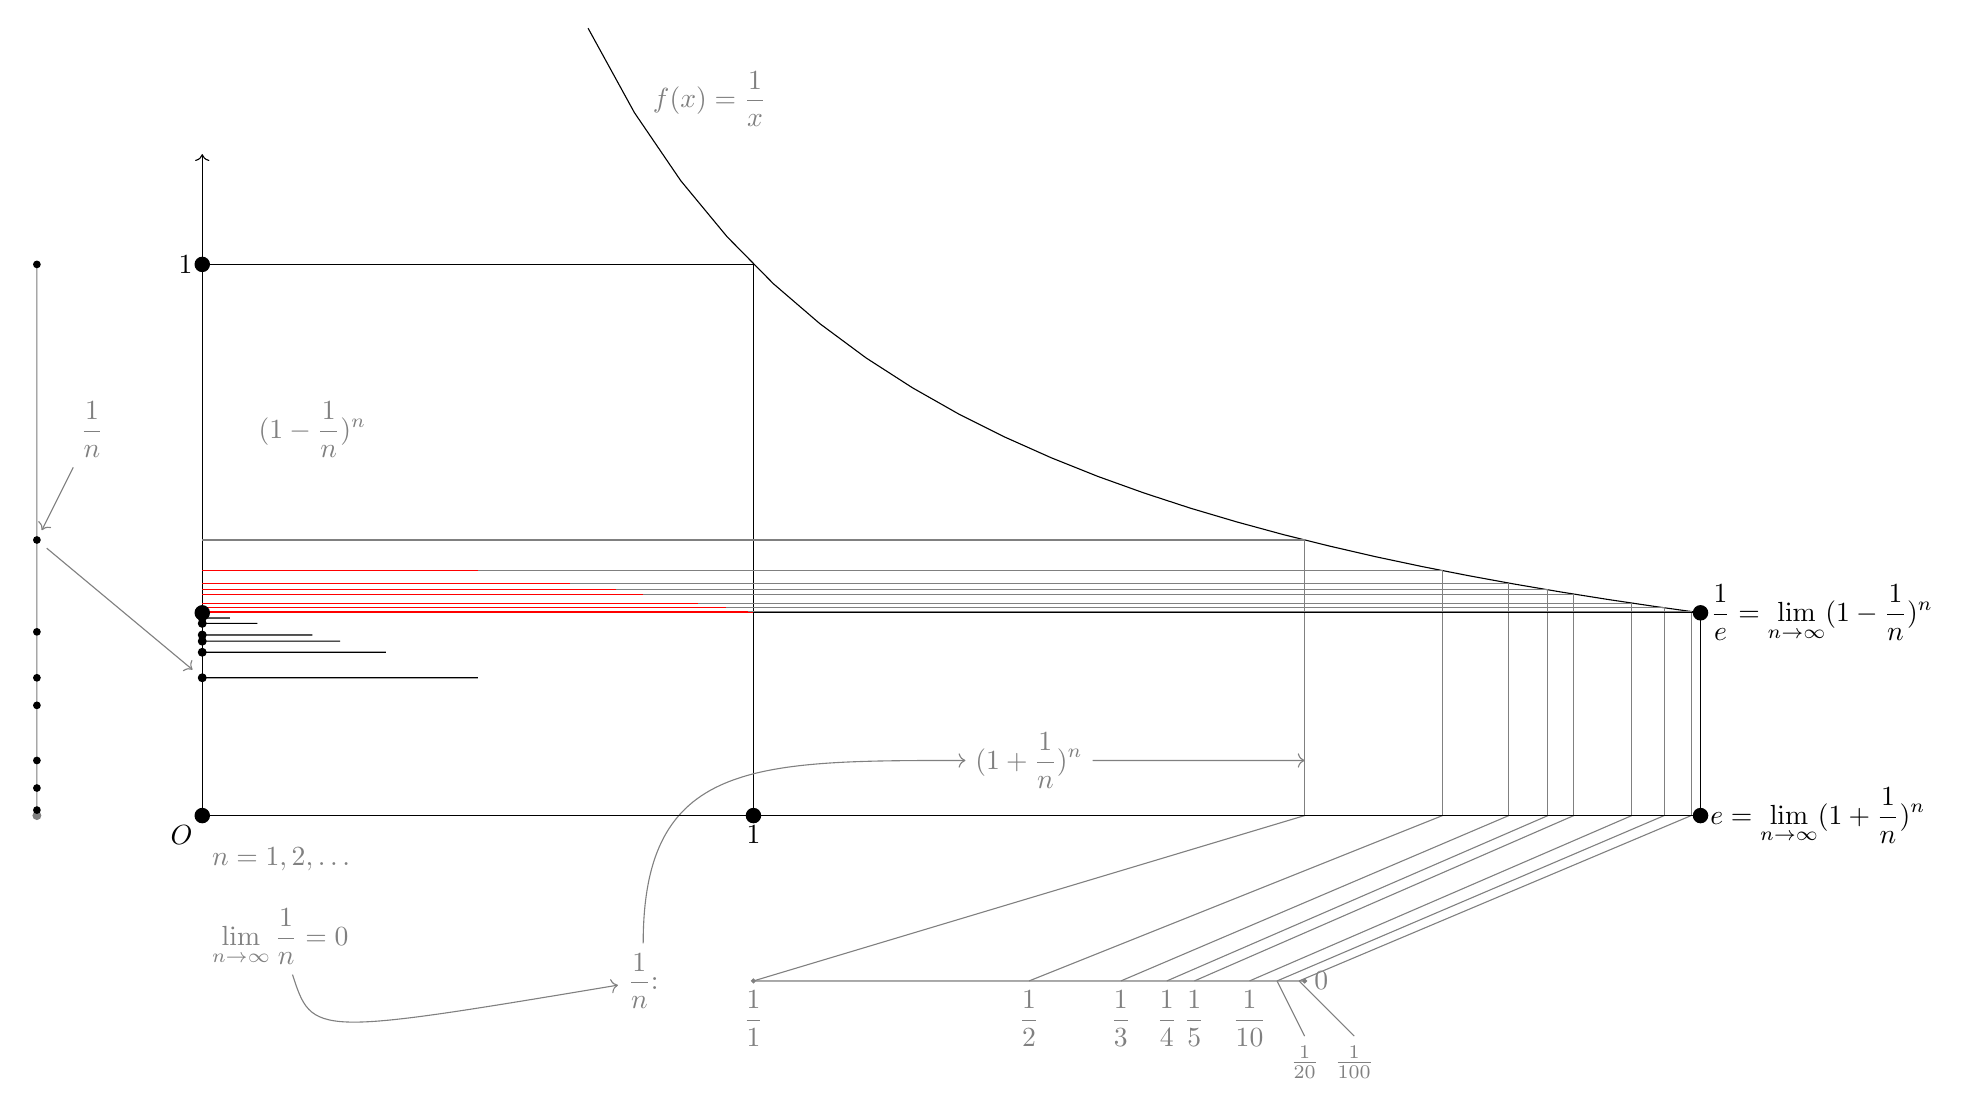
\begin{tikzpicture}[scale=7,domain=-.3:1.3]
%% \begin{tikzpicture}[xscale=5,xshift=-2,yscale=10,domain=-.3:1.3]

% \draw[very thin,color=gray] (-0.3,-0.3) grid (3.2,1.2);
%  \draw[->] (-1.2,0) -- (3.2,0) node[right] {$x$};
%  \draw[->] (0,-1.2) -- (0,2.2) node[above] {$f(x)$};

%%  f(x) = 1/x
  \draw[domain=.7:e,color=black] plot (\x,{(1/\x)});
  \draw[gray] (.8,1.3) node[right] {$f(x)=\displaystyle\frac{1}{x}$};

  %% axes
  \draw[->] (0,0) -- (0,1.2);

%% axis labels
%  \draw[black] (-0.1,.5) node %{\begin{sideways}$\displaystyle\lim_{n\to\infty}(1-\displaystyle\frac{1}{n})^n=\displaystyle\frac{1}{e}$\end{sideways}};

  \fill[black] (e,1/e) node[right]
  {$\displaystyle\frac{1}{e}=\lim_{n\to\infty}(1-\displaystyle\frac{1}{n})^n$} circle (.4pt);

  \fill[black] (e,0) node[right]
  {$e=\displaystyle\lim_{n\to\infty}(1+\frac{1}{n})^n$} circle (.4pt);

 %% dot (e,0)
%  \fill[black] (e,0) node[below] {$e$}
%  node[right=15pt] {$x=(1+\frac{1}{n})^n$}
%  circle (.4pt);


  %% indexing unit intervals
  %% horizontal
  \def\hidxv{-.3}
  \filldraw[gray] (1,\hidxv) circle (.1pt) %  node[left]  {$1$}
  -- (2,\hidxv) node[right] {$0$} circle (.1pt);

%% unit rectangles
  \draw[black] (0,0) rectangle (1,1);

% \draw[gray] (1,\hidxv) -- (2,0);
  \draw[gray] (0,\hidxv/2+0.07) node[right] (n) {$n=1,2,\dotsc$};
  \draw[gray] (0,\hidxv/2-0.07) node[right] (limninv) {$\displaystyle\lim_{n\rightarrow\infty}\frac{1}{n}=0$};
  \draw[gray] (.8,\hidxv) node (ninv) {$\displaystyle\frac{1}{n}$:};
%  -- (1,\hidxv/2)
  \draw[gray] (1.5,.1) node (eplus) {$\displaystyle (1+\frac{1}{n})^n$};
  \draw[->,gray] (eplus) -- (2,.1);

  \draw[->,gray] (limninv) .. controls (.2,-.4) .. (ninv);
  \draw[->,gray] (ninv) .. controls (.8,.1) and (1,.1) .. (eplus);

  \draw[gray] (1,\hidxv) node[below] {$\displaystyle\frac{1}{1}$} -- (2,0);

%  node[above,pos=.1] {\begin{turn}{45}$\displaystyle\frac{1}{n}\rightarrow (1+\frac{1}{n})^n$\end{turn}};
%  \draw[black] (2,0) node[below left] {$n=1$} -- (2,0);

  %% n=1
%  \draw[black] (0,0) rectangle (2,1/2); % n=1
 \draw[gray] (2,0) -- (2,1/2) -- (0,1/2);

  %% n=2
  \pgfmathsetmacro\term{(1+1/2)^2};
  \draw[gray] (\term,0) -- (\term,1/\term) -- (1-1/2,1/\term);
  \draw[color=red] (0,1/\term) -- (1-1/2,1/\term);

  \draw[gray] (1.5,\hidxv) node[below] {$\displaystyle\frac{1}{2}$} -- (\term,0);
%  \draw[gray] (1.5,\hidxv) -- (\term,0); % node[above=2pt,pos=.2]  {\begin{turn}{58}$(1+\frac{1}{2})^2$\end{turn}} ;

  %% n=3
  \pgfmathsetmacro\term{(1+1/3)^3};
  % \draw[black] (0,0) rectangle (\term,1/\term);
  \draw[gray] (\term,0) -- (\term,1/\term) -- (1-1/3,1/\term);
  \draw[color=red] (0,1/\term) -- (1-1/3,1/\term);
  \draw[gray] (2-1/3,\hidxv) node[below] {$\displaystyle\frac{1}{3}$}
  -- (\term,0); % node[above,pos=.2]  {\begin{turn}{60}$(1+\frac{1}{3})^3$\end{turn}} ;
%  \draw[black] (\term-0.03,-0.1) node[below left] {$(1+\frac{1}{3})^3$} -- (\term,0);

  \pgfmathsetmacro\term{(1+1/4)^4};
  \draw[gray] (\term,0) -- (\term,1/\term) -- (1-1/4,1/\term);
  \draw[color=red] (0,1/\term) -- (1-1/4,1/\term);
%  \draw[black] (0,0) rectangle (\term,1/\term);
  \draw[gray] (2-1/4,\hidxv) node[below] {$\displaystyle\frac{1}{4}$}
  -- (\term,0); % node[above,pos=.3]  {\begin{turn}{70}$(1+\frac{1}{4})^4$\end{turn}} ;

%  \draw[black] (\term-0.05,-0.2) node[below left] {$(1+\frac{1}{4})^4$}
%  --  (\term,0);
%  \draw[black] (-0.2,1/\term) node[left] {$(1+\frac{1}{4})^-4$} -- (0,1/\term);

  \pgfmathsetmacro\term{(1+1/5)^5};
  \draw[gray] (\term,0) -- (\term,1/\term) -- (1-1/5,1/\term);
  \draw[color=red] (0,1/\term) -- (1-1/5,1/\term);
%  \draw[black] (0,0) rectangle (\term,1/\term);
  \draw[gray] (2-1/5,\hidxv) node[below] {$\displaystyle\frac{1}{5}$}
  -- (\term,0); % node[above,pos=.3]  {\begin{turn}{60}$(1+\frac{1}{4})^4$\end{turn}} ;
%  \draw[black] (\term-0.05,-0.3) node[below] {$(1+\frac{1}{5})^5$}
%  --  (\term,0);

  \pgfmathsetmacro\term{(1+1/10)^10};
  \draw[gray] (\term,0) -- (\term,1/\term) -- (1-1/10,1/\term);
  \draw[color=red] (0,1/\term) -- (1-1/10,1/\term);
%  \draw[black] (0,0) rectangle (\term,1/\term);
  \draw[gray] (2-1/10,\hidxv) node[below] {$\displaystyle\frac{1}{10}$}
  -- (\term,0); % node[above,pos=.3]  {\begin{turn}{60}$(1+\frac{1}{4})^4$\end{turn}} ;
%  \draw[black] (\term,-0.4) node[below] {$(1+\frac{1}{10})^{10}$}
%  --  (\term,0);

  %% n=20
  \pgfmathsetmacro\term{(1+1/20)^20};
  \draw[gray] (\term,0) -- (\term,1/\term) -- (1-1/20,1/\term);
  \draw[color=red] (0,1/\term) -- (1-1/20,1/\term);
%  \draw[black] (0,0) rectangle (\term,1/\term);
  \draw[gray] (2-1/20,\hidxv) -- (\term,0);
  \draw[gray] (2-1/20+.05,\hidxv-.1) node[below] {$\frac{1}{20}$} -- (2-1/20,\hidxv);
  % node[above,pos=.3]  {\begin{turn}{60}$(1+\frac{1}{4})^4$\end{turn}} ;

  %% n=100
  \pgfmathsetmacro\term{(1+1/100)^100};
  \draw[gray] (\term,0) -- (\term,1/\term) -- (1-1/100,1/\term);
  \draw[color=red] (0,1/\term) -- (1-1/100,1/\term);
%  \draw[black] (0,0) rectangle (\term,1/\term);
  \draw[gray] (2-1/100,\hidxv) -- (\term,0);
  \draw[gray] (2-1/100+.1,\hidxv-.1) node[below] {$\frac{1}{100}$} -- (2-1/100,\hidxv);
%  \draw[black] (\term+0.1,1/\term+0.1) node[above] {$((1+\frac{1}{200})^{200},(1+\frac{1}{200})^{-200})$}
%  --  (\term,1/\term);

%%  n=infty
  \draw[black] (e,0) -- (e,1/e) -- (1,1/e);
  \draw[color=red] (0,1/e) -- (1,1/e);
  \draw[black] (0,0) -- (e,0);
%  \draw[black] (0,0) rectangle (e,1/e);

%  \draw[black] (0,1/e) -- (\e,1/e);
%  \fill[black] (0, 1/e) circle (.4pt) node[left]  {$\frac{1}{e}$};

  %% vertical
  \filldraw[gray] (-.3,0) circle (.2pt) -- (-.3,1);
  \draw[gray] (-.2,.7) node (vinv) {$\displaystyle\frac{1}{n}$};
  \draw[gray] (.2,.7) node (veinv)
  {$\displaystyle (1-\displaystyle\frac{1}{n})^n$};

  %% n=1
  \pgfmathsetmacro\term{(1-1/1)^1};
 \fill (-.3,1) node{} circle (.2pt);

 %% n=2
 \pgfmathsetmacro\term{(1-1/2)^2};
 \fill (-.3,1/2) node (vhalfidx) {} circle (.2pt);
 \filldraw (0,\term) node (vhalfax) {} circle (.2pt) -- (1/2,\term);
 \draw[->,gray] (vhalfidx) -- (vhalfax);
 \draw[->,gray] (vinv) -- (vhalfidx);
% \draw[->,gray] (veinv) -- (vhalfax);

 \pgfmathsetmacro\term{(1-1/3)^3};
 \fill (-.3,1/3) node{} circle (.2pt);
 \filldraw (0,\term) node {} circle (.2pt) -- (1/3,\term);
 
 \pgfmathsetmacro\term{(1-1/4)^4};
 \fill (-.3,1/4) node{} circle (.2pt);
 \filldraw (0,\term) node {} circle (.2pt) -- (1/4,\term);
 
 \pgfmathsetmacro\term{(1-1/5)^5};
 \fill (-.3,1/5) node{} circle (.2pt);
 \filldraw (0,\term) node {} circle (.2pt) -- (1/5,\term);

 \pgfmathsetmacro\term{(1-1/10)^10};
 \fill (-.3,1/10) node{} circle (.2pt);
 \filldraw (0,\term) node {} circle (.2pt) -- (1/10,\term);

 \pgfmathsetmacro\term{(1-1/20)^20};
 \fill (-.3,1/20) node{} circle (.2pt);
 \filldraw (0,\term) node {} circle (.2pt) -- (1/20,\term);

 \pgfmathsetmacro\term{(1-1/100)^100};
 \fill (-.3,1/100) node{} circle (.2pt);
 \filldraw (0,\term) node {} circle (.2pt) -- (1/100,\term);


  %% dot origin
  \fill[black] (0,0) node[below left] {$O$} circle (.4pt);

  %% dot (0,1/e)
 \fill[black] (0,1/e) circle (.4pt);

  %% dot (0,1)
  \fill[black] (0,1) node[left] {$1$} node[above right] {} circle (.4pt);
  %% dot (1,0)
  \fill[black] (1,0) node[below] {$1$} circle (.4pt);

%% label (1,e)
%  \fill[black] (1,e) node[anchor=south west] {$(1,e)$} circle (.4pt);

\end{tikzpicture}
\end{adjustbox}
\end{landscape}
\vfill
%%% Local Variables: 
%%% mode: latex
%%% TeX-master: t
%%% End: 

\include{hyperbolic.geometry.equilateral}
%%%%%%%%%%%%%%%%%%%%%%%%%%%%%%%%%%%%%%%%%%%%%%%%%%%%%%%%%%%%%%%%
%%  e Geometry 1
%%%%%%%%%%%%%%%%%%%%%%%%%%%%%%%%%%%%%%%%%%%%%%%%%%%%%%%%%%%%%%%%
\begin{figure}[ht]
  \center
  \caption{sweep e}
  \hspace*{-3cm}
\begin{tikzpicture}[scale=4,domain=-.3:1.3]

 \draw[very thin,color=gray] (-1,0) grid (3.2,1.2);
%  \draw[->] (-1.2,0) -- (3.2,0) node[right] {$x$};
%  \draw[->] (0,-1.2) -- (0,2.2) node[above] {$f(x)$};

  %% some ref lines
  \draw[gray] (1/\sqrttwo,0) node[color=black, below] {$\frac{1}{\sqrt{2}}$}
  -- (1/\sqrttwo,1/\sqrttwo);
  \draw[gray] (0,1/\sqrttwo) -- (1/\sqrttwo,1/\sqrttwo);

  %%%%%%%%%%%%%%%%
  % shade hyperbolic and circle sectors
  \begin{scope}[domain=1:e, even odd rule]
    \clip (0,0) -- (e,1/e) -- (1,1) -- cycle;
    \fill[color=blue,opacity=.15] (0,0) circle(1);

    \clip (0,0) circle(1) (0,0)--(1,1) -- plot (\x,{(1/\x)}) -- (e,1/e) -- cycle;
    \fill[opacity=.15] (0,0)--(1,1) -- plot (\x,{(1/\x)}) -- (e,1/e) -- cycle;
 \end{scope}

 %% axis:  f(x) = x
  \draw[color=gray] (0,0) -- (1.2,1.2) node[right] {$f(x) =x$};
  \draw[black] (0,0) -- (1,1);

  %% e diameter
  \draw[black] (0,0) -- (e,1/e);

%%%%%%%%%%%%%%%%
%% circle stuff
%%  unit circle
  \begin{scope}
    \clip (0,0) rectangle (1.1,1.1);
    \draw (0,0) circle (1);
   \end{scope}

 % 2.  circular rectilinear rotation
 %% dot endpts of arc
%\draw[-latex,red] (1/\sqrttwo,1/\sqrttwo) -- (1/\sqrttwo,\eeinv);
% \draw[-latex,red] (1/\sqrttwo,\eeinv) -- (1,\eeinv);

 % 3.  circular arc travel
 \begin{scope}
 \clip (0,0) -- (1,1) -- (e,1/e) -- cycle;
% \draw[thick,red] circle (1);
\end{scope}

\draw[gray] (1/\sqrttwo,1/\sqrttwo) -- (1,\eeinv); % NB: wrong x for
                                % pt 2

% 4. dots
% \fill[red] (1/\sqrttwo,1/\sqrttwo) node[above] {$A$} circle (.5pt);
% \fill[red] (1/\sqrttwo,\eeinv) node[left] {$B$} circle (.5pt);
% \fill[red] (1,\eeinv)  node[right] {$C$} circle (.5pt);


 %%%%%%%%%%%%%%%%
 % 1.  hyperbolic rectilinear rotation
  \draw[-latex,red] (1,1) -- (e,1);
  \draw[-latex,red] (e,1) -- (e,1/e);

%% f(x) = 1/x
  \draw[domain=.7:3.2,color=green!50!black] plot (\x,{(1/\x)});
  \draw[color=green!50!black] (.8,1.2) node[left] {$f(x) = \frac{1}{x}$};
  % \draw[] (1,.3) node[anchor=west] {$\scriptsize 1=\ln e$};
 %% 1/x travel

 %% chord
  \draw[black] (1,1) -- (e,1/e);

  %% arc
 \draw[-latex,thick,red,domain=1:e] plot (\x,{(1/\x)});

 %%%%%%%%%%%%%%%%

 %% moving vector
 \draw[-latex,black,postaction={decorate,
                    decoration={markings,
                      mark=at position 0.74 with {\arrow{latex}},
                      mark=at position 0.82 with {\arrow{latex}};}
                   }] (0,0) -- (1.8, 1);
\draw [->] (1.8,.975) -- (1.85,.975);

%%%%%%%%%%%%%%%%

 %% ref segments
  \draw[gray] (e,0) -- (e,1/e);

  \draw[gray] (-1,1/e) -- (e,1/e);
% \fill[black] (0, 1/e) circle (.7pt) node[left]  {$\frac{1}{e}$}
%  node[right] {$F$};



  %% (e,y) axis
%  \draw[red, dashed] (e,-1.1) -- (e, 3.9);
  %% (x,e) axis
%  \draw[red, dashed] (0,e) -- (3.9,e);

  %% (x,1) axis and label
%  \draw[red, dashed] (-0.1,1) -- (3.9,1);
%  \fill[black] (0,1) node[left] {$1$};

  %% secant
%  \draw[dashed] (0,0) -- (e, 1);


 %  \draw[gray] (1/\sqrttwo,0) node[below] {$\frac{1}{\sqrt{2}}$}
 %  -- (1/\sqrttwo,1/\sqrttwo);
 %  \draw[gray] (0,1/\sqrttwo) -- (1/\sqrttwo,1/\sqrttwo);

 %  \draw[gray] (\sqrttwo,0) node[below left] {$\scriptsize\sqrt{2}$}
 %  -- (\sqrttwo,\sqrttwo);
 %  \draw[gray] (0,\sqrttwo) -- (\sqrttwo,\sqrttwo);

 %  %%%%
 %  \draw[gray] (0,e/\sqrttwo) -- (e/\sqrttwo,e/\sqrttwo);
 % \draw[gray] (e/\sqrttwo,0) node[below] {$\frac{e}{\small\sqrt{2}}$}
 %  -- (e/\sqrttwo,e/\sqrttwo);

 %  %%%%
 %  \draw[gray] (0,3/2) node[left] {$\frac{3}{2}$} -- (3/2,3/2);
 %  \draw[gray] ({2-\sqrttwo+1},0) node[below=10pt] {$2-\frac{1}{e}$} -- ({2-\sqrttwo+1},{2-\sqrttwo+1});

  %% dot origin
  \fill[black] (0,0) node[below left] {$O$} circle (.7pt);

  %% dot (0,1/e)
 \fill[black] (0,1/e) circle (.7pt);

  %% dot (0,1)
  \fill[black] (0,1) node[left] {$1$} node[above right] {} circle (.7pt);
  %% dot (1,0)
  \fill[black] (1,0) node[below] {$1$} circle (.7pt);

  %% dot (1,1)
%  \fill[red] (1,1) node[above right] { $A'$}  circle (.5pt);

 %% label (1,e)
%  \fill[black] (1,e) node[anchor=south west] {$(1,e)$} circle (.7pt);

 %% dot (e,0)
  \fill[black] (e,0) node[below right]{$E$} node[below] {$e$} circle (.7pt);

  %% dot (e,1)
  \fill[red] (e,1) node[above right,color=red]  {$B'$} circle (.5pt); 

  %% dot (e,1/e)
  \fill[red] (e, 1/e) node[right] {$C'$} circle (.5pt);

  % \draw[green] (1,0) +(80:1cm) arc [radius=1cm,start angle=0];
  \draw (0,0) circle (1);
  \draw (1,0) circle (1);
  \draw (1,1) circle (1);

 \draw[thick,red] (1,0) arc [start angle=0,radius=1,end angle=deg(1)]
 node[black,above right] {$1$} -- (0,0);
 \draw[thick,red] (1,0) arc [start angle=0,radius=1,end angle=deg(2)]
 node[black,above left] {$2$} -- (0,0);

 \draw[thick,black] (1,0) arc [start angle=0,radius=1,end angle=deg(e)]
 node[black,left] {$e$} -- (0,0);
\draw[thick,black] (1,0) arc [start angle=0,radius=1,end angle=deg(e-2)]
 node[black,above right] {$e-2$} -- (0,0);
\draw[thick,black] (1,0) arc [start angle=0,radius=1,end angle=deg(pi/2-(e-2))]
 node[black,above right] {$\frac{\pi}{2}-e-2$} -- (0,0);
 \draw[thick,black] (1,0) arc [start angle=0,radius=1,end angle=deg(e-1)]
 node[black,above] {$e-1$} -- (0,0);
 \draw[thick,black] (1,0) arc [start angle=0,radius=1,end angle=deg(1-e)]
 node[black,below] {$1-e$} -- (0,0);

 \draw[thick,black] (1,0) arc [start angle=0,radius=1,end angle=deg(1/e)]
 node[black,right] {$1/e$} -- (0,0);
 \draw[thick,black] (1,0) arc [start angle=0,radius=1,end angle=deg(1-1/e)]
 node[black,right] {$1-1/e$} -- (0,0);

\end{tikzpicture}
\end{figure}


%%% Local Variables: 
%%% mode: latex
%%% TeX-master: t
%%% End: 

%%%%%%%%%%%%%%%%%%%%%%%%%%%%%%%%%%%%%%%%%%%%%%%%%%%%%%%%%%%%%%%%
%%  Hyperbolic Sector Geometry
%%%%%%%%%%%%%%%%%%%%%%%%%%%%%%%%%%%%%%%%%%%%%%%%%%%%%%%%%%%%%%%%
\begin{figure}[ht]
  \center
  \caption{sweep}
  \hspace*{-3cm}
  \begin{tikzpicture}[scale=5,domain=-.3:1.3]

    \draw[very thin,color=gray] (-0.3,-0.3) grid (3.2,1.2);
    %  \draw[->] (-1.2,0) -- (3.2,0) node[right] {$x$};
    %  \draw[->] (0,-1.2) -- (0,2.2) node[above] {$f(x)$};

    %% some ref lines
    \draw[gray] (1/\sqrttwo,0) node[color=black, below] {$\frac{1}{\sqrt{2}}$}
    -- (1/\sqrttwo,1/\sqrttwo);
    \draw[gray] (0,1/\sqrttwo) -- (1/\sqrttwo,1/\sqrttwo);

    %%%%%%%%%%%%%%%%
    % shade hyperbolic and circle sectors
    \begin{scope}[domain=1:e, even odd rule]
      \clip (0,0) -- (e,1/e) -- (1,1) -- cycle;
      \fill[color=blue,opacity=.15] (0,0) circle(1);

      \clip (0,0) circle(1) (0,0)--(1,1) -- plot (\x,{(1/\x)}) -- (e,1/e) -- cycle;
      \fill[opacity=.15] (0,0)--(1,1) -- plot (\x,{(1/\x)}) -- (e,1/e) -- cycle;
    \end{scope}

    %% axis:  f(x) = x
    \draw[color=gray] (0,0) -- (1.2,1.2) node[right] {$f(x) =x$};
    \draw[black] (0,0) -- (1,1);

    %% e diameter
    \draw[black] (0,0) -- (e,1/e);

    %%%%%%%%%%%%%%%%
    %% circle stuff
    %%  unit circle
    \begin{scope}
      \clip (0,0) rectangle (1.1,1.1);
      \draw (0,0) circle (1);
    \end{scope}

    % 2.  circular rectilinear rotation
    %% dot endpts of arc
    \draw[-latex,red] (1/\sqrttwo,1/\sqrttwo) -- (1/\sqrttwo,\eeinv);
    \draw[-latex,red] (1/\sqrttwo,\eeinv) -- (1,\eeinv);

    % 3.  circular arc travel
    \begin{scope}
      \clip (0,0) -- (1,1) -- (e,1/e) -- cycle;
      \draw[thick,red] circle (1);
    \end{scope}

    \draw[gray] (1/\sqrttwo,1/\sqrttwo) -- (1,\eeinv); % NB: wrong x for
    % pt 2

    % 4. dots
    \fill[red] (1/\sqrttwo,1/\sqrttwo) node[above] {$A$} circle (.5pt);
    \fill[red] (1/\sqrttwo,\eeinv) node[left] {$B$} circle (.5pt);
    \fill[red] (1,\eeinv)  node[right] {$C$} circle (.5pt);


    %%%%%%%%%%%%%%%%
    % 1.  hyperbolic rectilinear rotation
    \draw[-latex,red] (1,1) -- (e,1);
    \draw[-latex,red] (e,1) -- (e,1/e);

    %% f(x) = 1/x
    \draw[domain=.7:3.2,color=green!50!black] plot (\x,{(1/\x)});
    \draw[color=green!50!black] (.85,1.2) node[right] {$f(x) = \frac{1}{x}$};
    % \draw[] (1,.3) node[anchor=west] {$\scriptsize 1=\ln e$};
    %% 1/x travel

    %% chord
    \draw[black] (1,1) -- (e,1/e);

    %% plotted arc
    \draw[-latex,thick,red,domain=1:e] plot (\x,{(1/\x)});

    %%%%%%%%%%%%%%%%

    %% moving vector
    \draw[-latex,black,postaction={decorate,
        decoration={markings,
          mark=at position 0.74 with {\arrow{latex}},
          mark=at position 0.82 with {\arrow{latex}};}
    }] (0,0) -- (1.8, 1);
    \draw [->] (1.8,.975) -- (1.85,.975);

    %%%%%%%%%%%%%%%%

    %% ref segments
    \draw[gray] (e,0) -- (e,1/e);

    \draw[gray] (0,1/e) -- (e,1/e);
    \fill[black] (0, 1/e) circle (.7pt) node[left]  {$\frac{1}{e}$}
    node[right] {$F$};



    %% (e,y) axis
    %  \draw[red, dashed] (e,-1.1) -- (e, 3.9);
    %% (x,e) axis
    %  \draw[red, dashed] (0,e) -- (3.9,e);

    %% (x,1) axis and label
    %  \draw[red, dashed] (-0.1,1) -- (3.9,1);
    %  \fill[black] (0,1) node[left] {$1$};

    %% secant
    %  \draw[dashed] (0,0) -- (e, 1);


    %  \draw[gray] (1/\sqrttwo,0) node[below] {$\frac{1}{\sqrt{2}}$}
    %  -- (1/\sqrttwo,1/\sqrttwo);
    %  \draw[gray] (0,1/\sqrttwo) -- (1/\sqrttwo,1/\sqrttwo);

    %  \draw[gray] (\sqrttwo,0) node[below left] {$\scriptsize\sqrt{2}$}
    %  -- (\sqrttwo,\sqrttwo);
    %  \draw[gray] (0,\sqrttwo) -- (\sqrttwo,\sqrttwo);

    %  %%%%
    %  \draw[gray] (0,e/\sqrttwo) -- (e/\sqrttwo,e/\sqrttwo);
    % \draw[gray] (e/\sqrttwo,0) node[below] {$\frac{e}{\small\sqrt{2}}$}
    %  -- (e/\sqrttwo,e/\sqrttwo);

    %  %%%%
    %  \draw[gray] (0,3/2) node[left] {$\frac{3}{2}$} -- (3/2,3/2);
    %  \draw[gray] ({2-\sqrttwo+1},0) node[below=10pt] {$2-\frac{1}{e}$} -- ({2-\sqrttwo+1},{2-\sqrttwo+1});

    %% dot origin
    \fill[black] (0,0) node[below left] {$O$} circle (.7pt);

    %% dot (0,1/e)
    \fill[black] (0,1/e) circle (.7pt);

    %% dot (0,1)
    \fill[black] (0,1) node[left] {$1$} node[above right] {} circle (.7pt);
    %% dot (1,0)
    \fill[black] (1,0) node[below] {$1$} circle (.7pt);

    %% dot (1,1)
    \fill[red] (1,1) node[above right] { $A'$}  circle (.5pt);

    %% label (1,e)
    %  \fill[black] (1,e) node[anchor=south west] {$(1,e)$} circle (.7pt);

    %% dot (e,0)
    \fill[black] (e,0) node[below right]{$E$} node[below] {$e$} circle (.7pt);

    %% dot (e,1)
    \fill[red] (e,1) node[above right,color=red]  {$B'$} circle (.5pt); 

    %% dot (e,1/e)
    \fill[red] (e, 1/e) node[right] {$C'$} circle (.5pt);

    %% dot (e, e)
    %  \fill[red] (e, e) circle (.7pt) node[below right]  {$(e,e)$};

    %  \draw[<-] (e, .7) -- (e+.4,.7) node[anchor=west] {$1-\frac{1}{e}$};
    % \fill[black] (1,e) node[anchor=south west] {$(1,e)$} circle (.7pt);

    % \draw (e,0) arc (0:90:e);
    % \fill (canvas polar cs:angle=45,radius=2.71cm) circle (.7pt)
    % node[right] {$P$};
    % \fill (canvas polar cs:angle=30,radius=2.71cm)
    % node[right]{$\frac{\pi\,e}{4} = PE$};

    %  \fill (0,e) circle (.7pt) node[anchor=east] {($0,e$)};

    %% dot (0, 1/e)
    %  \fill[black] (1, 1/e) circle (.7pt);
    %% dot (e, 1/e)

  \end{tikzpicture}
\end{figure}

%%% Local Variables: 
%%% mode: latex
%%% TeX-master: t
%%% End: 

%%%%%%%%%%%%%%%%%%%%%%%%%%%%%%%%%%%%%%%%%%%%%%%%%%%%%%%%%%%%%%%%
%%  HOMOTHETIC TRANSFORM
%%%%%%%%%%%%%%%%%%%%%%%%%%%%%%%%%%%%%%%%%%%%%%%%%%%%%%%%%%%%%%%%
\begin{animateinline}[%
    poster=first%
    %% ,draft
    %% ,loop
    ,controls%
  ]{\the\value{iFrameRate}}%

  %%%%  INITIAL FRAME REQUIRED in order to get n+1 frames (good starts and ends)
  %% \begin{tikzpicture}
  %%   \useasboundingbox[draw] {(-1,-2) rectangle (10,16)};
  %% \end{tikzpicture}
  %% \newframe
  %%%% MULTIFRAMES START FROM 1 NOT 0
  \multiframe{\value{iFrames}}{iFrame=1+1}{%
    \message{\iFrame}

    \begin{tikzpicture}[%
        scale=\tikzscale
      ]%
      %% \if usebb
      	%% \useasboundingbox[\bbdraw] {(\bbminx,\bbminy) rectangle (\bbmaxx,\bbmaxy)};
      %% \fi

      \tkzInit[ymin=\tkzminy,ymax=\tkzmaxy,xmin=\tkzminx,xmax=\tkzmaxx]
      \tkzGrid
      \tkzAxeXY
      \tkzClip

      \tkzDefPoint(0,0){O}
      \tkzDefPoint(1,0){I}
      \tkzDefPointBy[homothety=center O ratio  10 ](I)  \tkzGetPoint{A}
      \tkzDefMidPoint(O,A)              \tkzGetPoint{M}
      \tkzDefPointWith[orthogonal](I,M) \tkzGetPoint{H}
      \tkzInterLC(I,H)(M,A)             \tkzGetSecondPoint{B}

      \tkzDrawSegment(O,A)
      \tkzDrawSegment[style=dashed](I,H)
      \tkzDrawPoints(O,I,A,B,M)
      \tkzDrawArc(M,A)(O)
      \tkzMarkRightAngle(A,I,B)

      \tkzLabelSegment[right=4pt](I,B){$\sqrt{a}$}
      \tkzLabelSegment[below](O,I){$1$}
      \tkzLabelSegment[below](I,M){$a/2$}
      \tkzLabelSegment[below](M,A){$a/2$}
      \tkzLabelPoints(I,M,B,A)
      \tkzLabelPoint[below left](O){$O$}
    \end{tikzpicture}

  }% multiframe
\end{animateinline}

%%% Local Variables:
%%% mode: latex
%%% TeX-master: t
%%% End:

%%%%%%%%%%%%%%%%%%%%%%%%%%%%%%%%%%%%%%%%%%%%%%%%%%%%%%%%%%%%%%%%
%%  SWEEP
%%%%%%%%%%%%%%%%%%%%%%%%%%%%%%%%%%%%%%%%%%%%%%%%%%%%%%%%%%%%%%%%
\begin{figure}[ht]
  \center
  \caption{sweep}
  \hspace*{-3cm}
\begin{tikzpicture}[scale=5,domain=-.3:1.3]

 \draw[very thin,color=gray] (-0.3,-0.3) grid (3.2,1.2);
%  \draw[->] (-1.2,0) -- (3.2,0) node[right] {$x$};
%  \draw[->] (0,-1.2) -- (0,2.2) node[above] {$f(x)$};

  %% some ref lines
  \draw[gray] (1/\sqrttwo,0) node[color=black, below] {$\frac{1}{\sqrt{2}}$}
  -- (1/\sqrttwo,1/\sqrttwo);
  \draw[gray] (0,1/\sqrttwo) -- (1/\sqrttwo,1/\sqrttwo);

  %%%%%%%%%%%%%%%%
  % shade hyperbolic and circle sectors
  \begin{scope}[domain=1:\e, even odd rule]
    \clip (0,0) -- (e,1/e) -- (1,1) -- cycle;
    \fill[color=blue,opacity=.15] (0,0) circle(1);

    \clip (0,0) circle(1) (0,0)--(1,1) -- plot (\x,{(1/\x)}) -- (\e,\inve) -- cycle;
    \fill[opacity=.15] (0,0)--(1,1) -- plot (\x,{(1/\x)}) -- (\e,\inve) -- cycle;
 \end{scope}

 %% axis:  f(x) = x
  \draw[color=gray] (0,0) -- (1.2,1.2) node[right] {$f(x) =x$};
  \draw[black] (0,0) -- (1,1);

  %% e diameter
  \draw[black] (0,0) -- (e,1/e);

%%%%%%%%%%%%%%%%
%% circle stuff
%%  unit circle
  \begin{scope}
    \clip (0,0) rectangle (1.1,1.1);
    \draw (0,0) circle (1);
   \end{scope}

 % 2.  circular rectilinear rotation
 %% dot endpts of arc
\draw[-latex,red] (1/\sqrttwo,1/\sqrttwo) -- (1/\sqrttwo,\esqinv);
 \draw[-latex,red] (1/\sqrttwo,\esqinv) -- (1,\esqinv);

 % 3.  circular arc travel
 \begin{scope}
 \clip (0,0) -- (1,1) -- (e,1/e) -- cycle;
 \draw[thick,red] circle (1);
\end{scope}

\draw[gray] (1/\sqrttwo,1/\sqrttwo) -- (1,\esqinv); % NB: wrong x for
                                % pt 2

% 4. dots
 \fill[red] (1/\sqrttwo,1/\sqrttwo) node[above] {$A$} circle (.5pt);
 \fill[red] (1/\sqrttwo,\esqinv) node[left] {$B$} circle (.5pt);
 \fill[red] (1,\esqinv)  node[right] {$C$} circle (.5pt);


 %%%%%%%%%%%%%%%%
 % 1.  hyperbolic rectilinear rotation
  \draw[-latex,red] (1,1) -- (e,1);
  \draw[-latex,red] (e,1) -- (e,1/e);

%% f(x) = 1/x
  \draw[domain=.7:3.2,color=green!50!black] plot (\x,{(1/\x)});
  \draw[color=green!50!black] (.85,1.2) node[right] {$f(x) = \frac{1}{x}$};
  % \draw[] (1,.3) node[anchor=west] {$\scriptsize 1=\ln e$};
 %% 1/x travel

 %% chord
  \draw[black] (1,1) -- (e,1/e);

  %% plotted arc
 \draw[-latex,thick,red,domain=1:e] plot (\x,{(1/\x)});

 %%%%%%%%%%%%%%%%

 %% moving vector
 \draw[-latex,black,postaction={decorate,
                    decoration={markings,
                      mark=at position 0.74 with {\arrow{latex}},
                      mark=at position 0.82 with {\arrow{latex}};}
                   }] (0,0) -- (1.8, 1);
\draw [->] (1.8,.975) -- (1.85,.975);

%%%%%%%%%%%%%%%%

 %% ref segments
  \draw[gray] (e,0) -- (e,1/e);

  \draw[gray] (0,\inve) -- (\e,\inve);
 \fill[black] (0, \inve) circle (.7pt) node[left]  {$\frac{1}{e}$}
  node[right] {$F$};



  %% (e,y) axis
%  \draw[red, dashed] (\e,-1.1) -- (\e, 3.9);
  %% (x,e) axis
%  \draw[red, dashed] (0,\e) -- (3.9,\e);

  %% (x,1) axis and label
%  \draw[red, dashed] (-0.1,1) -- (3.9,1);
%  \fill[black] (0,1) node[left] {$1$};

  %% secant
%  \draw[dashed] (0,0) -- (\e, 1);


 %  \draw[gray] (1/\sqrttwo,0) node[below] {$\frac{1}{\sqrt{2}}$}
 %  -- (1/\sqrttwo,1/\sqrttwo);
 %  \draw[gray] (0,1/\sqrttwo) -- (1/\sqrttwo,1/\sqrttwo);

 %  \draw[gray] (\sqrttwo,0) node[below left] {$\scriptsize\sqrt{2}$}
 %  -- (\sqrttwo,\sqrttwo);
 %  \draw[gray] (0,\sqrttwo) -- (\sqrttwo,\sqrttwo);

 %  %%%%
 %  \draw[gray] (0,e/\sqrttwo) -- (e/\sqrttwo,e/\sqrttwo);
 % \draw[gray] (e/\sqrttwo,0) node[below] {$\frac{e}{\small\sqrt{2}}$}
 %  -- (e/\sqrttwo,e/\sqrttwo);

 %  %%%%
 %  \draw[gray] (0,3/2) node[left] {$\frac{3}{2}$} -- (3/2,3/2);
 %  \draw[gray] ({2-\sqrttwo+1},0) node[below=10pt] {$2-\frac{1}{e}$} -- ({2-\sqrttwo+1},{2-\sqrttwo+1});

  %% dot origin
  \fill[black] (0,0) node[below left] {$O$} circle (.7pt);

  %% dot (0,1/e)
 \fill[black] (0,\inve) circle (.7pt);

  %% dot (0,1)
  \fill[black] (0,1) node[left] {$1$} node[above right] {} circle (.7pt);
  %% dot (1,0)
  \fill[black] (1,0) node[below] {$1$} circle (.7pt);

  %% dot (1,1)
  \fill[red] (1,1) node[above right] { $A'$}  circle (.5pt);

 %% label (1,e)
%  \fill[black] (1,\e) node[anchor=south west] {$(1,e)$} circle (.7pt);

 %% dot (e,0)
  \fill[black] (\e,0) node[below right]{$E$} node[below] {$e$} circle (.7pt);

  %% dot (e,1)
  \fill[red] (\e,1) node[above right,color=red]  {$B'$} circle (.5pt); 

  %% dot (e,1/e)
  \fill[red] (\e, \inve) node[right] {$C'$} circle (.5pt);

 %% dot (e, e)
%  \fill[red] (\e, e) circle (.7pt) node[below right]  {$(e,e)$};

%  \draw[<-] (\e, .7) -- (\e+.4,.7) node[anchor=west] {$1-\frac{1}{e}$};
  % \fill[black] (1,\e) node[anchor=south west] {$(1,e)$} circle (.7pt);

% \draw (\e,0) arc (0:90:\e);
% \fill (canvas polar cs:angle=45,radius=2.71cm) circle (.7pt)
% node[right] {$P$};
% \fill (canvas polar cs:angle=30,radius=2.71cm)
% node[right]{$\frac{\pi\,e}{4} = PE$};

%  \fill (0,\e) circle (.7pt) node[anchor=east] {($0,e$)};

  %% dot (0, 1/e)
%  \fill[black] (1, \inve) circle (.7pt);
 %% dot (e, 1/e)

\end{tikzpicture}
\end{figure}

%%% Local Variables: 
%%% mode: latex
%%% TeX-master: t
%%% End: 

%%%%%%%%%%%%%%%%%%%%%%%%%%%%%%%%%%%%%%%%%%%%%%%%%%%%%%%%%%%%%%%%
%% Hyperbolic Rotation 1
%% simple circular and hyperbolic rotation - sweep of radius
%%%%%%%%%%%%%%%%%%%%%%%%%%%%%%%%%%%%%%%%%%%%%%%%%%%%%%%%%%%%%%%%
\pgfmathparse{\value{iFrameRate}}
\begin{animateinline}[%
    poster=first%
    %% ,draft
    %% ,loop
    ,controls%
  ]{\pgfmathresult}%

  %%%%  INITIAL FRAME REQUIRED in order to get n+1 frames (good starts and ends)

  %% \begin{tikzpicture}
  %%   \useasboundingbox[draw] {(-1,-2) rectangle (10,16)};

  %% \end{tikzpicture}
  %% \newframe

  %%%% MULTIFRAMES START FROM 1 NOT 0
  \multiframe{\pgfmathresult}{iFrame=1+1}{%
    %% \message{\iFrame}
    %% \message{\arabic{iFrames}}
    %% \message{\rFromXa}
    %% \message{\rToXa}
    %% \message{\rFromXb}
    %% \message{\rToXb}

    \pgfmathsetmacro\xa{easeInQuadratic(\iFrame,\rFromXa,\rDeltaXa,\value{iFrames})};
    \pgfmathsetmacro\xb{easeInQuadratic(\iFrame,\rFromXb,\rDeltaXb,\value{iFrames})};
    %% \pgfmathsetmacro\newx{easeInQuadratic(\iFrame,\rFromXa,\rDeltaXa,\value{iFrames})};

    \begin{tikzpicture}[%
        scale=\tikzscale
        %% ,domain=-.3:1.3
      ]
      %% \if usebb
      \useasboundingbox[\bbdraw] {(\bbminx,\bbminy) rectangle (\bbmaxx,\bbmaxy)};
      %% \fi


      \draw[very thin,color=gray] (-1,0) grid (3.2,1.2);

      %% axis of symmetry:  f(x) = x
      \draw[<->,color=gray] (-1,-1) -- (1.2,1.2) node[right] {$f(x) =x$};
      \draw[black] (0,0) -- (1,1);

      %% e diameter
      \draw[black] (0,0) -- (e,1/e);

      %% %% coordinate rectangle
      %% \begin{scope}[domain=1:e, even odd rule]
      %%   \draw[ultra thick,black,domain=1:e] (0,0) -- (0,{1/\xa}) -- (\xa,{1/\xa}) -- (\xa,0) -- cycle;
      %%   \clip[domain=1:e] (0,0) -- (0,{1/\xa}) -- (\xa,{1/\xa}) -- (\xa,0) -- cycle;
      %%   \draw[pattern=horizontal lines light blue] (0,0) rectangle (e,1);
      %% \end{scope}

      %%  unit circle
      \begin{scope}
        %% \clip (0,0) rectangle (1.1,1.1);
        \draw (0,0) circle (1);
      \end{scope}

      %% ref segments
      \draw[gray] (e,0) -- (e,1/e);

      \draw[gray] (0,1/e) node[left] {$e^{-1}$} -- (e,1/e);

      \draw[gray] (0,.5) node[left] {$0.5$} -- (e,.5);

      %% dot origin
      \fill[black] (0,0) node[below left] {$O$} circle (.4pt);

      %% dot (0,1/e)
      \fill[black] (0,1/e) circle (.4pt);

      %% dot (0,1)
      \fill[black] (0,1) node[above left] {$1$} {} circle (.4pt);
      %% dot (1,0)
      \fill[black] (1,0) node[below right] {$1$} circle (.4pt);

      %% dot (e,0)
      \fill[black] (e,0) node[below] {$e$} circle (.4pt) -- (e,1.2);

      %% e area
      \begin{scope}[domain=1:e, even odd rule]
        \clip[domain=\xa:\xb] (1,0) --  plot (\xa,{(1/\xa)}) -- (\xa,0) -- cycle;
        \draw[pattern=vertical lines,pattern color=blue] (0,0) rectangle (e,1);
      \end{scope}

      %% hyperbolic sector
      \begin{scope}[domain=1:e, even odd rule]
        \clip[domain=1:\xa] (0,0) --  plot (\xa,{(1/\xa)}) -- cycle;
        \fill[color=green!50!blue,opacity=.15] (0,0) rectangle (e,1);
      \end{scope}

      %% f(x) = 1/x
      \draw[<->,domain=.7:3.2,color=green!50!black] plot (\xa,{(1/\xa)});
      \draw[color=green!50!black] (.8,1.2) node[left] {$f(x) = \frac{1}{x}$};

      %% hyperbolic arc
      \draw[thick,red,domain=1:\xa] plot (\x,{(1/\x)});
      %% hyperbolic radii
      \draw[very thick] (1,0) -- (1,1);
      \draw[semithick] (0,0) -- (\xa,1/\xa);

      %%%%%%%%%%%%%%%%

      %% sweeping vector
      %%  \draw[-latex,black,postaction={decorate,
      %%                     decoration={markings,
      %%                       mark=at position 0.74 with {\arrow{latex}},
      %%                       mark=at position 0.82 with {\arrow{latex}};}
      %%                    }] (0,0) -- (1.8, 1);
      %% \draw [->] (1.8,.975) -- (1.85,.975);

      %%%%%%%%%%%%%%%%
    \end{tikzpicture}
  }% multiframe
\end{animateinline}

%%% Local Variables: 
%%% mode: latex
%%% TeX-master: t
%%% End: 

%%%%%%%%%%%%%%%%%%%%%%%%%%%%%%%%%%%%%%%%%%%%%%%%%%%%%%%%%%%%%%%%
%%  SWEEP e
%%%%%%%%%%%%%%%%%%%%%%%%%%%%%%%%%%%%%%%%%%%%%%%%%%%%%%%%%%%%%%%%
\begin{animateinline}[poster=first,loop]{\value{iFrameRate}}%
    %% ,draft

    %% ,controls%
  %% ]
  %%%%  INITIAL FRAME REQUIRED in order to get n+1 frames (good starts and ends)
  %% \begin{tikzpicture}
  %%   \useasboundingbox[draw] {(-1,-2) rectangle (10,16)};
  %% \end{tikzpicture}
  %% \newframe
  %%%% MULTIFRAMES START FROM 1 NOT 0
  \multiframe{\value{iFrames}}{%
    iFrame=0+1
  }{%
    \message{\iFrame}

    \begin{tikzpicture}[%
        scale=\tikzscale
        ,domain=-.3:7.4%
      ]
      %% \if usebb
      \useasboundingbox[\bbdraw]{(\bbminx,\bbminy) rectangle (\bbmaxx,\bbmaxy)};
      %% \fi

      %%%%%%%%%%%%%%%%%%%%%%%%%%%%%%%%%%%%%%%%%%%%%%%%%%%%%%%%%%%%%%%%

      %% grid
      \draw[very thin,gray!50] (0,0) grid (e^2+.2,2.2);
      %% axes
      \draw[<->,black] (-.2,0) -- (e^2+.2,0);
      \draw[<->,black] (0,-.2) -- (0,2.2);

      %% ref segments
      \draw[gray] (0,.5) node[left] {} -- (.1,.5);
      %% dot (0,0.5)
      %% \fill[gray] (0,.5) node[left] {$0.5$} circle (.4pt);

      %% dot origin
      %% \fill[black] (0,0) node[below left] {$0$} circle (.4pt);

      %% dot (0,1/e)
      %% \fill[black] (0,\inve) circle (.4pt);

      %% log scale
      \fill[black] (-1,0) node[below] {$logarithmic:$};
      \fill[black] (1,0) node[below] {$0$};
      \fill[black] (e,0) node[below] {$1$};
      \draw[black] (e,0) -- (e,2.2);
      \fill[black] (e^2,0) node[below] {$2$};
      \draw[black] (e^2,0) -- (e^2,2.2);

      \fill[gray] (-1,-.5) node {$arithmetic:$};
      \fill[gray] (0,-.5) node {$0$};
      \fill[gray] (1,-.5) node {$1$};
      \fill[gray] (2,-.5) node {$2$};
      \fill[gray] (e,-.5) node {$e^1$};
      \fill[gray] (3,-.5) node {$3$};
      \fill[gray] (4,-.5) node {$4$};
      \fill[gray] (5,-.5) node {$5$};
      \fill[gray] (6,-.5) node {$6$};
      \fill[gray] (7,-.5) node {$7$};
      \fill[gray] (e^2,-.5) node {$e^2$};


      %%%%%%%%%%%%%%%%
      %% % 1.  hyperbolic rectilinear rotation
      %% \draw[-latex,red] (1,1) -- (e,1);
      %% \draw[-latex,red] (e,1) -- (e,1/e);

      %% hyperbolic rotation animation
      \begin{scope}[even odd rule]
        \pgfmathsetmacro\xa{easeInQuadratic(\iFrame,\rFromXa,\rDeltaXa,\value{iFrames})};
        \pgfmathsetmacro\xb{easeInQuadratic(\iFrame,\rFromXb,\rDeltaXb,\value{iFrames})};
        %% shade unit square
        \fill[gray,opacity=.2] (0,0) rectangle (1,1);
        %% shade unit rectangle
        \draw[pattern=horizontal lines light blue] (0,0) rectangle (\xb,1/\xb);
        \draw (0,1/\xb) node[left] {$e^n$} -- (\xb,1/\xb);
        %% shade rotated region - source
        \begin{scope}
          \clip[samples=100,domain=\xa:\xb] (\xa,0) -- plot (\x,{(1/\x)}) -- (\xb,0) -- cycle ;
          \fill[green,opacity=.25] (0,0) rectangle (e^2,1);
        \end{scope}
        %% shade rotated region - destination
        \begin{scope}
          \pgfmathsetmacro\samps{1-\iFrame/\value{iFrames}}
          \clip[samples=100*\samps,domain=\xb:\rToXb*.9]
          (\xb,0) -- plot (\x,{(1/\x)}) -- (e^2,1/e^2) -- (e^2,0) -- cycle;
          %% (\xb,0) -- (\xb,{(1/\xb)}) -- (\rToXb,1/\rToXb) -- (\rToXb,0) -- cycle;
          \draw[opacity=.5,pattern=crosshatch dots light steel blue] (0,0) rectangle (e^2,1);
        \end{scope}
        %% f(x) = 1/x
        \draw[>->,samples=100,domain=.4:e^2+.2,color=green!50!black] plot (\x,{(1/\x)});
        \draw[color=green!50!black] (.5,1/.5) node[above right] {$f(x) = \frac{1}{x}$};
        %% border rotated region
        \draw[green!50!black,very thick,samples=100,domain=\xa:\xb]
        (\xa,0) -- plot (\x,{(1/\x)}) -- (\xb,0) -- cycle ;
        %% area labels
        \draw (3.5,.7) node[above] (area) {area = $1$};
        %% label of rotated region - source
        \draw[->] (area)
        .. controls +(down:12pt) and +(up:12pt) .. ({\xa+(\xb-\xa)*.2},{(1/\xa)*.5});
        %% label of unit square
        \draw[->] (area) .. controls +(left:36pt) and +(up:24pt) .. (.5,.5);
        %% label of unit rectangle
        \draw[->] (area) .. controls +(left:36pt) and +(up:24pt) .. (\xa/2,{(1/\xa)*.2});
        %% label of rotated region - destination
        \draw[->,opacity=(1-\iFrame/\value{iFrames})] (area)
        .. controls +(right:12pt) and +(up:12pt) .. (4.5,.1);
      \end{scope}
    \end{tikzpicture}
  }% multiframe
\end{animateinline}

%%% Local Variables: 
%%% mode: latex
%%% TeX-master: t
%%% End: 

%%%%%%%%%%%%%%%%%%%%%%%%%%%%%%%%%%%%%%%%%%%%%%%%%%%%%%%%%%%%%%%%
%% Hyperbolic Rotation 3
%% sliding projection area
%%%%%%%%%%%%%%%%%%%%%%%%%%%%%%%%%%%%%%%%%%%%%%%%%%%%%%%%%%%%%%%%
\pgfmathparse{\value{iFrameRate}}
\begin{animateinline}[%
    poster=first%
    %% ,draft
    %% ,loop
    ,controls%
  ]{\the\value{iFrameRate}}%

  %%%%  INITIAL FRAME REQUIRED in order to get n+1 frames (good starts and ends)

  %% \begin{tikzpicture}
  %%   \useasboundingbox[draw] {(-1,-2) rectangle (10,16)};

  %% \end{tikzpicture}
  %% \newframe

  %%%% MULTIFRAMES START FROM 1 NOT 0
  \multiframe{\value{iFrameRate}}{iFrame=1+1}{%
    %% \message{\arabic{iFrames}}
    %% \message{\iFrame}
    %% \message{\rFromXa}
    %% \message{\rToXa}
    %% \message{\rFromXb}
    %% \message{\rToXb}

    \begin{tikzpicture}[%
        scale=\tikzscale
        ,domain=-.3:7.4%
      ]
      %% \if usebb
      \useasboundingbox[\bbdraw]{(\bbminx,\bbminy) rectangle (\bbmaxx,\bbmaxy)};
      %% \fi

      \pgfmathsetmacro\xa{easeInQuadratic(\iFrame,\rFromXa,\rDeltaXa,\value{iFrames})};
      \pgfmathsetmacro\xb{easeInQuadratic(\iFrame,\rFromXb,\rDeltaXb,\value{iFrames})};

      %% grid
      \draw[very thin,gray!50] (0,0) grid (e^2+.2,2.2);
      %% axes
      \draw[<->,black] (-.2,0) -- (e^2+.2,0);
      \draw[<->,black] (0,-.2) -- (0,2.2);

      %% ref segments
      \draw[gray] (0,.5) node[left] {} -- (.1,.5);
      %% dot (0,0.5)
      %% \fill[gray] (0,.5) node[left] {$0.5$} circle (.4pt);

      %% dot origin
      %% \fill[black] (0,0) node[below left] {$0$} circle (.4pt);

      %% dot (0,1/e)
      %% \fill[black] (0,\inve) circle (.4pt);

      %% log scale
      \fill[black] (-1,0) node[below] {$logarithmic:$};
      \fill[black] (1,0) node[below] {$0$};
      \fill[black] (e,0) node[below] {$1$};
      \draw[black] (e,0) -- (e,2.2);
      \fill[black] (e^2,0) node[below] {$2$};
      \draw[black] (e^2,0) -- (e^2,2.2);

      \fill[gray] (-1,-.5) node {$arithmetic:$};
      \fill[gray] (0,-.5) node {$0$};
      \fill[gray] (1,-.5) node {$1$};
      \fill[gray] (2,-.5) node {$2$};
      \fill[gray] (e,-.5) node {$e^1$};
      \fill[gray] (3,-.5) node {$3$};
      \fill[gray] (4,-.5) node {$4$};
      \fill[gray] (5,-.5) node {$5$};
      \fill[gray] (6,-.5) node {$6$};
      \fill[gray] (7,-.5) node {$7$};
      \fill[gray] (e^2,-.5) node {$e^2$};

      %%%%%%%%%%%%%%%%
      %% % 1.  hyperbolic rectilinear rotation
      %% \draw[-latex,red] (1,1) -- (e,1);
      %% \draw[-latex,red] (e,1) -- (e,1/e);

      %% hyperbolic rotation animation
      \begin{scope}[even odd rule]
        %% shade unit square
        \fill[gray,opacity=.2] (0,0) rectangle (1,1);
        %% coordinate rectangle
        \draw[pattern=horizontal lines light blue] (0,0) rectangle (\xb,1/\xb);
        \draw (0,1/\xb) node[left] {$e^n$} -- (\xb,1/\xb);
        %% shade rotated region - source
        \begin{scope}
          \clip[samples=100,domain=\xa:\xb] (\xa,0) -- plot (\x,{(1/\x)}) -- (\xb,0) -- cycle ;
          \fill[green,opacity=.25] (0,0) rectangle (e^2,1);
        \end{scope}
        %% shade rotated region - destination
        \begin{scope}
          \pgfmathsetmacro\samps{1-\iFrame/\value{iFrames}}
          \clip[samples=100*\samps,domain=\xb:\rToXb*.9]
          (\xb,0) -- plot (\x,{(1/\x)}) -- (e^2,1/e^2) -- (e^2,0) -- cycle;
          %% (\xb,0) -- (\xb,{(1/\xb)}) -- (\rToXb,1/\rToXb) -- (\rToXb,0) -- cycle;
          \draw[opacity=.5,pattern=crosshatch dots light steel blue] (0,0) rectangle (e^2,1);
        \end{scope}
        %% f(x) = 1/x
        \draw[>->,samples=100,domain=.4:e^2+.2,color=green!50!black] plot (\x,{(1/\x)});
        \draw[color=green!50!black] (.5,1/.5) node[above right] {$f(x) = \frac{1}{x}$};
        %% border rotated region
        \draw[green!50!black,very thick,samples=100,domain=\xa:\xb]
        (\xa,0) -- plot (\x,{(1/\x)}) -- (\xb,0) -- cycle ;
        %% area labels
        \draw (3.5,.7) node[above] (area) {area = $1$};
        %% label of rotated region - source
        \draw[->] (area)
        .. controls +(down:12pt) and +(up:12pt) .. ({\xa+(\xb-\xa)*.2},{(1/\xa)*.5});
        %% label of unit square
        \draw[->] (area) .. controls +(left:36pt) and +(up:24pt) .. (.5,.5);
        %% label of unit rectangle
        \draw[->] (area) .. controls +(left:36pt) and +(up:24pt) .. (\xa/2,{(1/\xa)*.2});
        %% label of rotated region - destination
        \draw[->,opacity=(1-\iFrame/\value{iFrames})] (area)
        .. controls +(right:12pt) and +(up:12pt) .. (4.5,.1);
      \end{scope}
    \end{tikzpicture}
  }% multiframe
\end{animateinline}

%%% Local Variables: 
%%% mode: latex
%%% TeX-master: t
%%% End: 

%%%%%%%%%%%%%%%%%%%%%%%%%%%%%%%%%%%%%%%%%%%%%%%%%%%%%%%%%%%%%%%%
%% Hyperbolic Rotation 4
%% trapezoidal and coord rect slide (dup of 3)
%%%%%%%%%%%%%%%%%%%%%%%%%%%%%%%%%%%%%%%%%%%%%%%%%%%%%%%%%%%%%%%%
\begin{animateinline}[%
    poster=first%
    %% ,draft
    %% ,loop
    ,controls%
  ]{\the\value{iFrameRate}}%

  %% %%%%  INITIAL FRAME REQUIRED in order to get n+1 frames (good starts and ends)

  %% \begin{tikzpicture}
  %%   \useasboundingbox[draw] {(-1,-2) rectangle (10,16)};

  %% \end{tikzpicture}
  %% %% \newframe

  %%%% MULTIFRAMES START FROM 1 NOT 0
  \multiframe{\value{iFrameRate}}{iFrame=0+1}{%
    \message{\iFrame}
    %% \message{\arabic{iFrames}}
    %% \message{\rFromXa}
    %% \message{\rToXa}
    %% \message{\rFromXb}
    %% \message{\rToXb}

    \begin{tikzpicture}[%
        scale=\tikzscale
        ,domain=-.3:7.4%
      ]
  %%     %% \if usebb
      \useasboundingbox[\bbdraw]{(\bbminx,\bbminy) rectangle (\bbmaxx,\bbmaxy)};
  %%     %% \fi


      \pgfmathsetmacro\xa{easeInQuadratic(\iFrame,\rFromXa,\rDeltaXa,\value{iFrames})};
      \pgfmathsetmacro\xb{easeInQuadratic(\iFrame,\rFromXb,\rDeltaXb,\value{iFrames})};

      %% grid
      \draw[very thin,gray!50] (0,0) grid (e^2+.2,2.2);
      %% axes
      \draw[<->,black] (-.2,0) -- (e^2+.2,0);
      \draw[<->,black] (0,-.2) -- (0,2.2);

      %% ref segments
      \draw[gray] (0,.5) node[left] {} -- (.1,.5);
      %% dot (0,0.5)
      %% \fill[gray] (0,.5) node[left] {$0.5$} circle (.4pt);

      %% dot origin
      %% \fill[black] (0,0) node[below left] {$0$} circle (.4pt);

      %% dot (0,1/e)
      %% \fill[black] (0,\inve) circle (.4pt);

      %% log scale
      \fill[black] (-1,0) node[below] {$logarithmic:$};
      \fill[black] (1,0) node[below] {$0$};
      \fill[black] (e,0) node[below] {$1$};
      \draw[black] (e,0) -- (e,2.2);
      \fill[black] (e^2,0) node[below] {$2$};
      \draw[black] (e^2,0) -- (e^2,2.2);

      \fill[gray] (-1,-.5) node {$arithmetic:$};
      \fill[gray] (0,-.5) node {$0$};
      \fill[gray] (1,-.5) node {$1$};
      \fill[gray] (2,-.5) node {$2$};
      \fill[gray] (e,-.5) node {$e^1$};
      \fill[gray] (3,-.5) node {$3$};
      \fill[gray] (4,-.5) node {$4$};
      \fill[gray] (5,-.5) node {$5$};
      \fill[gray] (6,-.5) node {$6$};
      \fill[gray] (7,-.5) node {$7$};
      \fill[gray] (e^2,-.5) node {$e^2$};
      %%%%%%%%%%%%%%%%
      %% % 1.  hyperbolic rectilinear rotation
      %% \draw[-latex,red] (1,1) -- (e,1);
      %% \draw[-latex,red] (e,1) -- (e,1/e);

  %%     %% hyperbolic rotation animation
      \begin{scope}[even odd rule]
        %% shade unit square
        \fill[gray,opacity=.2] (0,0) rectangle (1,1);
        %% coordinate rectangle
        \draw[pattern=horizontal lines light blue] (0,0) rectangle (\xb,1/\xb);
        \draw (0,1/\xb) node[left] {$e^n$} -- (\xb,1/\xb);
        %% shade rotated region - source
        \begin{scope}
          \clip[samples=100,domain=\xa:\xb] (\xa,0) -- plot (\x,{(1/\x)}) -- (\xb,0) -- cycle ;
          \fill[green,opacity=.25] (0,0) rectangle (e^2,1);
        \end{scope}
        %% shade rotated region - destination
        \begin{scope}
          \pgfmathsetmacro\samps{1-\iFrame/\value{iFrames}}
          \clip[samples=100*\samps,domain=\xb:\rToXb*.9]
          (\xb,0) -- plot (\x,{(1/\x)}) -- (e^2,1/e^2) -- (e^2,0) -- cycle;
          %% (\xb,0) -- (\xb,{(1/\xb)}) -- (\rToXb,1/\rToXb) -- (\rToXb,0) -- cycle;
          \draw[opacity=.5,pattern=crosshatch dots light steel blue] (0,0) rectangle (e^2,1);
        \end{scope}
        %% f(x) = 1/x
        \draw[>->,samples=100,domain=.4:e^2+.2,color=green!50!black] plot (\x,{(1/\x)});
        \draw[color=green!50!black] (.5,1/.5) node[above right] {$f(x) = \frac{1}{x}$};
        %% border rotated region
        \draw[green!50!black,very thick,samples=100,domain=\xa:\xb]
        (\xa,0) -- plot (\x,{(1/\x)}) -- (\xb,0) -- cycle ;
        %% area labels
        \draw (3.5,.7) node[above] (area) {area = $1$};
        %% label of rotated region - source
        \draw[->] (area)
        .. controls +(down:12pt) and +(up:12pt) .. ({\xa+(\xb-\xa)*.2},{(1/\xa)*.5});
        %% label of unit square
        \draw[->] (area) .. controls +(left:36pt) and +(up:24pt) .. (.5,.5);
        %% label of unit rectangle
        \draw[->] (area) .. controls +(left:36pt) and +(up:24pt) .. (\xa/2,{(1/\xa)*.2});
        %% label of rotated region - destination
        \draw[->,opacity=(1-\iFrame/\value{iFrames})] (area)
        .. controls +(right:12pt) and +(up:12pt) .. (4.5,.1);
      \end{scope}
    \end{tikzpicture}
  }% multiframe
\end{animateinline}

%%% Local Variables: 
%%% mode: latex
%%% TeX-master: t
%%% End: 

%%%%%%%%%%%%%%%%%%%%%%%%%%%%%%%%%%%%%%%%%%%%%%%%%%%%%%%%%%%%%%%%
%% Hyperbolic Rotation - oops. 
%% three-move ``rotation''
%% TODO:  rotate a single point
%%%%%%%%%%%%%%%%%%%%%%%%%%%%%%%%%%%%%%%%%%%%%%%%%%%%%%%%%%%%%%%%
\begin{animateinline}[%
    poster=first%
    %% ,draft
    %% ,loop
    ,controls%
  ]{\the\value{iFrameRate}}%

  %%%%  INITIAL FRAME REQUIRED in order to get n+1 frames (good starts and ends)

  %% \begin{tikzpicture}
  %%   \useasboundingbox[draw] {(-1,-2) rectangle (10,16)};

  %% \end{tikzpicture}
  %% \newframe

  %%%% MULTIFRAMES START FROM 1 NOT 0
  \multiframe{\value{iFrames}}{iFrame=1+1}{%
    %% \message{\arabic{iFrames}}
    %% \message{\iFrame}
    %% \message{\rFromXa}
    %% \message{\rToXa}
    %% \message{\rFromXb}
    %% \message{\rToXb}

    \begin{tikzpicture}[%
        scale=\tikzscale
        ,domain=-.3:7.4%
      ]
      %% \if usebb
      \useasboundingbox[\bbdraw]{(\bbminx,\bbminy) rectangle (\bbmaxx,\bbmaxy)};
      %% \fi

      \pgfmathsetmacro\xa{easeInQuadratic(\iFrame,\rFromXa,\rDeltaXa,\value{iFrames})};
      \pgfmathsetmacro\xb{easeInQuadratic(\iFrame,\rFromXb,\rDeltaXb,\value{iFrames})};

      %% grid
      \draw[very thin,gray!50] (0,0) grid (e^2+.2,7);
      %% axes
      \draw[<->,black] (-.2,0) -- (e^2+.2,0);
      \draw[<->,black] (0,-.2) -- (0,2.2);

      %% ref segments
      \draw[gray] (0,.5) node[left] {} -- (.1,.5);
      %% dot (0,0.5)
      %% \fill[gray] (0,.5) node[left] {$0.5$} circle (.4pt);

      %% dot origin
      %% \fill[black] (0,0) node[below left] {$0$} circle (.4pt);

      %% dot (0,1/e)
      %% \fill[black] (0,\inve) circle (.4pt);

      %% log scale
      \fill[black] (-1,0) node[below] {$logarithmic:$};
      \fill[black] (1,0) node[below] {$0$};
      \fill[black] (e,0) node[below] {$1$};
      \draw[black] (e,0) -- (e,2.2);
      \fill[black] (e^2,0) node[below] {$2$};
      \draw[black] (e^2,0) -- (e^2,2.2);

      \fill[gray] (-1,-.5) node {$arithmetic:$};
      \fill[gray] (0,-.5) node {$0$};
      \fill[gray] (1,-.5) node {$1$};
      \fill[gray] (2,-.5) node {$2$};
      \fill[gray] (e,-.5) node {$e^1$};
      \fill[gray] (3,-.5) node {$3$};
      \fill[gray] (4,-.5) node {$4$};
      \fill[gray] (5,-.5) node {$5$};
      \fill[gray] (6,-.5) node {$6$};
      \fill[gray] (7,-.5) node {$7$};
      \fill[gray] (e^2,-.5) node {$e^2$};

      %% v axis labels
      \fill[->,gray] (0,e) node {$e^1$} -- (e^2+.2,e);

      %%%%%%%%%%%%%%%%
      %% % 1.  hyperbolic rectilinear rotation
      %% \draw[-latex,red] (1,1) -- (e,1);
      %% \draw[-latex,red] (e,1) -- (e,1/e);

      %% hyperbolic rotation animation
      \begin{scope}[even odd rule]
        %% %% shade unit square
        %% \fill[gray,opacity=.2] (0,0) rectangle (1,1);
        %% %% coordinate rectangle
        %% \draw[pattern=horizontal lines light blue] (0,0) rectangle (\xb,1/\xb);
        %% \draw (0,1/\xb) node[left] {$e^n$} -- (\xb,1/\xb);

        %% shade rotated region - source
        %% \begin{scope}
        %%   \clip[samples=100,domain=1:e] (1,0) -- plot (\x,1/\x+e*(1/\x)) -- (\xb,0) -- cycle ;
        %%   \fill[green,opacity=.25] (0,0) rectangle (e^2,1);
        %% \end{scope}

        %% \draw[red,samples=100,domain=1:e] plot (\x,{1/\x+(e-1/\x)*\xa}); % (e-1/\x)*pct

        \pgfmathsetmacro\pct{\iFrame/\value{iFrames}}

        %% \draw[red,dashed,samples=100,domain=1:e] plot (\x,1/\x);

        %% \draw[red,dashed,samples=100,domain=1:e] plot (\x,{1+1/\x+((e-1)/\x)});

        %%%%%%%%%%%%%%%%
        \draw[<->,green!10!black,samples=100,domain=.5:e^2+.2]
        plot (\x,{1/\x+\pct*(1+(e-1)/\x)});

        %% lower left to upper left

        \draw[green!50!black,ultra thick,samples=100,domain=1:e]
        (1,\pct) -- plot (\x,{1/\x+\pct*(1+(e-1)/\x)})
        -- (e,\pct) -- cycle;

        %% %% shade rotated region - destination
        %% \begin{scope}
        %%   \pgfmathsetmacro\samps{1-\iFrame/\value{iFrames}}
        %%   \clip[samples=100*\samps,domain=\xb:\rToXb*.9]
        %%   (\xb,0) -- plot (\x,{(1/\x)}) -- (e^2,1/e^2) -- (e^2,0) -- cycle;
        %%   %% (\xb,0) -- (\xb,{(1/\xb)}) -- (\rToXb,1/\rToXb) -- (\rToXb,0) -- cycle;
        %%   \draw[opacity=.5,pattern=crosshatch dots light steel blue] (0,0) rectangle (e^2,1);
        %% \end{scope}
        %% %% f(x) = 1/x
        %% \draw[>->,samples=100,domain=.4:e^2+.2,color=green!50!black] plot (\x,{(1/\x)});
        %% \draw[color=green!50!black] ({((e^2)-.5)},{1/((e^2)-.5)}) node[above left] {$f(x) = \frac{1}{x}$};
        %% %% border rotated region
        %% \draw[green!50!black,very thick,samples=100,domain=\xa:\xb]
        %% (\xa,0) -- plot (\x,{(1/\x)}) -- (\xb,0) -- cycle ;
        %% %% area labels
        %% \draw (3.5,.7) node[above] (area) {area = $1$};
        %% %% label of rotated region - source
        %% \draw[->] (area)
        %% .. controls +(down:12pt) and +(up:12pt) .. ({\xa+(\xb-\xa)*.2},{(1/\xa)*.5});
        %% %% label of unit square
        %% \draw[->] (area) .. controls +(left:36pt) and +(up:24pt) .. (.5,.5);
        %% %% label of unit rectangle
        %% \draw[->] (area) .. controls +(left:36pt) and +(up:24pt) .. (\xa/2,{(1/\xa)*.2});
        %% %% label of rotated region - destination
        %% \draw[->,opacity=(1-\iFrame/\value{iFrames})] (area)
        %% .. controls +(right:12pt) and +(up:12pt) .. (4.5,.1);
      \end{scope}
    \end{tikzpicture}
  }% multiframe

  \newframe*
  %%%%%%%%%%%%%%%%%%%%%%%%%%%%%%%%%%%%%%%%%%%%%%%%%%%%%%%%%%%%%%%%
  %% STEP 2:  upper left to upper right
  \multiframe{\value{iFrames}}{iFrame=1+1}{%
    %% \message{\arabic{iFrames}}
    %% \message{\iFrame}
    %% \message{\rFromXa}
    %% \message{\rToXa}
    %% \message{\rFromXb}
    %% \message{\rToXb}

    \begin{tikzpicture}[%
        scale=\tikzscale
        ,domain=-.3:7.4%
      ]
      %% \if usebb
      \useasboundingbox[\bbdraw]{(\bbminx,\bbminy) rectangle (\bbmaxx,\bbmaxy)};
      %% \fi

      \pgfmathsetmacro\xa{easeInQuadratic(\iFrame,\rFromXa,\rDeltaXa,\value{iFrames})};
      \pgfmathsetmacro\xb{easeInQuadratic(\iFrame,\rFromXb,\rDeltaXb,\value{iFrames})};

      %% grid
      \draw[very thin,gray!50] (0,0) grid (e^2+.2,7);
      %% axes
      \draw[<->,black] (-.2,0) -- (e^2+.2,0);
      \draw[<->,black] (0,-.2) -- (0,2.2);

      %% ref segments
      \draw[gray] (0,.5) node[left] {} -- (.1,.5);
      %% dot (0,0.5)
      %% \fill[gray] (0,.5) node[left] {$0.5$} circle (.4pt);

      %% dot origin
      %% \fill[black] (0,0) node[below left] {$0$} circle (.4pt);

      %% dot (0,1/e)
      %% \fill[black] (0,\inve) circle (.4pt);

      %% log scale
      \fill[black] (-1,0) node[below] {$logarithmic:$};
      \fill[black] (1,0) node[below] {$0$};
      \fill[black] (e,0) node[below] {$1$};
      \draw[black] (e,0) -- (e,2.2);
      \fill[black] (e^2,0) node[below] {$2$};
      \draw[black] (e^2,0) -- (e^2,2.2);

      \fill[gray] (-1,-.5) node {$arithmetic:$};
      \fill[gray] (0,-.5) node {$0$};
      \fill[gray] (1,-.5) node {$1$};
      \fill[gray] (2,-.5) node {$2$};
      \fill[gray] (e,-.5) node {$e^1$};
      \fill[gray] (3,-.5) node {$3$};
      \fill[gray] (4,-.5) node {$4$};
      \fill[gray] (5,-.5) node {$5$};
      \fill[gray] (6,-.5) node {$6$};
      \fill[gray] (7,-.5) node {$7$};
      \fill[gray] (e^2,-.5) node {$e^2$};

      %% v axis labels
      \fill[->,gray] (0,e) node {$e^1$} -- (e^2+.2,e);

      %%%%%%%%%%%%%%%%
      %% % 1.  hyperbolic rectilinear rotation
      %% \draw[-latex,red] (1,1) -- (e,1);
      %% \draw[-latex,red] (e,1) -- (e,1/e);

      %% hyperbolic rotation animation
      \begin{scope}[even odd rule]
        %% %% shade unit square
        %% \fill[gray,opacity=.2] (0,0) rectangle (1,1);
        %% %% coordinate rectangle
        %% \draw[pattern=horizontal lines light blue] (0,0) rectangle (\xb,1/\xb);
        %% \draw (0,1/\xb) node[left] {$e^n$} -- (\xb,1/\xb);

        %% shade rotated region - source
        %% \begin{scope}
        %%   \clip[samples=100,domain=1:e] (1,0) -- plot (\x,1/\x+e*(1/\x)) -- (\xb,0) -- cycle ;
        %%   \fill[green,opacity=.25] (0,0) rectangle (e^2,1);
        %% \end{scope}

        %% \draw[red,samples=100,domain=1:e] plot (\x,{1/\x+(e-1/\x)*\xa}); % (e-1/\x)*pct

        \pgfmathsetmacro\pct{\iFrame/\value{iFrames}}

        %% \draw[red,dashed,samples=100,domain=1:e] plot (\x,1/\x);

        %% \draw[red,dashed,samples=100,domain=1:e] plot (\x,{1+1/\x+((e-1)/\x)});

        \draw[<->,green!10!black,samples=100,domain=.5:e^2+.2]
        	plot (\x,{1/\x+(1+(e-1)/\x)});

                %% upper left to upper right
        \draw[green!50!black,ultra thick,samples=100,domain=\xa:\xb]
        	(\xa,1) -- plot (\x,{1/\x+(1+(e-1)/\x)})
        	-- (\xb,1) -- cycle;

        %% %% shade rotated region - destination
        %% \begin{scope}
        %%   \pgfmathsetmacro\samps{1-\iFrame/\value{iFrames}}
        %%   \clip[samples=100*\samps,domain=\xb:\rToXb*.9]
        %%   (\xb,0) -- plot (\x,{(1/\x)}) -- (e^2,1/e^2) -- (e^2,0) -- cycle;
        %%   %% (\xb,0) -- (\xb,{(1/\xb)}) -- (\rToXb,1/\rToXb) -- (\rToXb,0) -- cycle;
        %%   \draw[opacity=.5,pattern=crosshatch dots light steel blue] (0,0) rectangle (e^2,1);
        %% \end{scope}
        %% %% f(x) = 1/x
        %% \draw[>->,samples=100,domain=.4:e^2+.2,color=green!50!black] plot (\x,{(1/\x)});
        %% \draw[color=green!50!black] ({((e^2)-.5)},{1/((e^2)-.5)}) node[above left] {$f(x) = \frac{1}{x}$};
        %% %% border rotated region
        %% \draw[green!50!black,very thick,samples=100,domain=\xa:\xb]
        %% (\xa,0) -- plot (\x,{(1/\x)}) -- (\xb,0) -- cycle ;
        %% %% area labels
        %% \draw (3.5,.7) node[above] (area) {area = $1$};
        %% %% label of rotated region - source
        %% \draw[->] (area)
        %% .. controls +(down:12pt) and +(up:12pt) .. ({\xa+(\xb-\xa)*.2},{(1/\xa)*.5});
        %% %% label of unit square
        %% \draw[->] (area) .. controls +(left:36pt) and +(up:24pt) .. (.5,.5);
        %% %% label of unit rectangle
        %% \draw[->] (area) .. controls +(left:36pt) and +(up:24pt) .. (\xa/2,{(1/\xa)*.2});
        %% %% label of rotated region - destination
        %% \draw[->,opacity=(1-\iFrame/\value{iFrames})] (area)
        %% .. controls +(right:12pt) and +(up:12pt) .. (4.5,.1);
      \end{scope}
    \end{tikzpicture}
  }% multiframe

  \newframe*
  %%%%%%%%%%%%%%%%%%%%%%%%%%%%%%%%%%%%%%%%%%%%%%%%%%%%%%%%%%%%%%%%
  %% STEP 3:  upper right to lower right
  %%%%%%%%%%%%%%%%%%%%%%%%%%%%%%%%%%%%%%%%%%%%%%%%%%%%%%%%%%%%%%%%
  \multiframe{\value{iFrames}}{iFrame=1+1}{%
    %% \message{\arabic{iFrames}}
    %% \message{\iFrame}
    %% \message{\rFromXa}
    %% \message{\rToXa}
    %% \message{\rFromXb}
    %% \message{\rToXb}

    \begin{tikzpicture}[%
        scale=\tikzscale
        ,domain=-.3:7.4%
      ]
      %% \if usebb
      \useasboundingbox[\bbdraw]{(\bbminx,\bbminy) rectangle (\bbmaxx,\bbmaxy)};
      %% \fi

      \pgfmathsetmacro\xa{easeInQuadratic(\iFrame,\rFromXa,\rDeltaXa,\value{iFrames})};
      \pgfmathsetmacro\xb{easeInQuadratic(\iFrame,\rFromXb,\rDeltaXb,\value{iFrames})};

      %% grid
      \draw[very thin,gray!50] (0,0) grid (e^2+.2,7);
      %% axes
      \draw[<->,black] (-.2,0) -- (e^2+.2,0);
      \draw[<->,black] (0,-.2) -- (0,2.2);

      %% ref segments
      \draw[gray] (0,.5) node[left] {} -- (.1,.5);
      %% dot (0,0.5)
      %% \fill[gray] (0,.5) node[left] {$0.5$} circle (.4pt);

      %% dot origin
      %% \fill[black] (0,0) node[below left] {$0$} circle (.4pt);

      %% dot (0,1/e)
      %% \fill[black] (0,\inve) circle (.4pt);

      %% log scale
      \fill[black] (-1,0) node[below] {$logarithmic:$};
      \fill[black] (1,0) node[below] {$0$};
      \fill[black] (e,0) node[below] {$1$};
      \draw[black] (e,0) -- (e,2.2);
      \fill[black] (e^2,0) node[below] {$2$};
      \draw[black] (e^2,0) -- (e^2,2.2);

      \fill[gray] (-1,-.5) node {$arithmetic:$};
      \fill[gray] (0,-.5) node {$0$};
      \fill[gray] (1,-.5) node {$1$};
      \fill[gray] (2,-.5) node {$2$};
      \fill[gray] (e,-.5) node {$e^1$};
      \fill[gray] (3,-.5) node {$3$};
      \fill[gray] (4,-.5) node {$4$};
      \fill[gray] (5,-.5) node {$5$};
      \fill[gray] (6,-.5) node {$6$};
      \fill[gray] (7,-.5) node {$7$};
      \fill[gray] (e^2,-.5) node {$e^2$};

      %% v axis labels
      \fill[->,gray] (0,e) node {$e^1$} -- (e^2+.2,e);

      %%%%%%%%%%%%%%%%
      %% % 1.  hyperbolic rectilinear rotation
      %% \draw[-latex,red] (1,1) -- (e,1);
      %% \draw[-latex,red] (e,1) -- (e,1/e);

      %% hyperbolic rotation animation
      \begin{scope}[even odd rule]
        %% %% shade unit square
        %% \fill[gray,opacity=.2] (0,0) rectangle (1,1);
        %% %% coordinate rectangle
        %% \draw[pattern=horizontal lines light blue] (0,0) rectangle (\xb,1/\xb);
        %% \draw (0,1/\xb) node[left] {$e^n$} -- (\xb,1/\xb);

        %% shade rotated region - source
        %% \begin{scope}
        %%   \clip[samples=100,domain=1:e] (1,0) -- plot (\x,1/\x+e*(1/\x)) -- (\xb,0) -- cycle ;
        %%   \fill[green,opacity=.25] (0,0) rectangle (e^2,1);
        %% \end{scope}

        %% \draw[red,samples=100,domain=1:e] plot (\x,{1/\x+(e-1/\x)*\xa}); % (e-1/\x)*pct

        \pgfmathsetmacro\pct{\iFrame/\value{iFrames}}

        %% \draw[red,dashed,samples=100,domain=1:e] plot (\x,1/\x);

        %% \draw[red,dashed,samples=100,domain=1:e] plot (\x,{1+1/\x+((e-1)/\x)});

        \draw[<->,green!10!black,samples=100,domain=.5:e^2+.2]
        	plot (\x,{1/\x+(1-\pct+(e-1)/\x)});

%% upper right to lower left
        \draw[green!50!black,ultra thick,samples=100,domain=e:e^2]
        	(e,1-\pct) -- plot (\x,{1/\x+(1-\pct+(e-1)/\x)})
        	-- (e^2,1-\pct) -- cycle;

        %% %% shade rotated region - destination
        %% \begin{scope}
        %%   \pgfmathsetmacro\samps{1-\iFrame/\value{iFrames}}
        %%   \clip[samples=100*\samps,domain=\xb:\rToXb*.9]
        %%   (\xb,0) -- plot (\x,{(1/\x)}) -- (e^2,1/e^2) -- (e^2,0) -- cycle;
        %%   %% (\xb,0) -- (\xb,{(1/\xb)}) -- (\rToXb,1/\rToXb) -- (\rToXb,0) -- cycle;
        %%   \draw[opacity=.5,pattern=crosshatch dots light steel blue] (0,0) rectangle (e^2,1);
        %% \end{scope}
        %% %% f(x) = 1/x
        %% \draw[>->,samples=100,domain=.4:e^2+.2,color=green!50!black] plot (\x,{(1/\x)});
        %% \draw[color=green!50!black] ({((e^2)-.5)},{1/((e^2)-.5)}) node[above left] {$f(x) = \frac{1}{x}$};
        %% %% border rotated region
        %% \draw[green!50!black,very thick,samples=100,domain=\xa:\xb]
        %% (\xa,0) -- plot (\x,{(1/\x)}) -- (\xb,0) -- cycle ;
        %% %% area labels
        %% \draw (3.5,.7) node[above] (area) {area = $1$};
        %% %% label of rotated region - source
        %% \draw[->] (area)
        %% .. controls +(down:12pt) and +(up:12pt) .. ({\xa+(\xb-\xa)*.2},{(1/\xa)*.5});
        %% %% label of unit square
        %% \draw[->] (area) .. controls +(left:36pt) and +(up:24pt) .. (.5,.5);
        %% %% label of unit rectangle
        %% \draw[->] (area) .. controls +(left:36pt) and +(up:24pt) .. (\xa/2,{(1/\xa)*.2});
        %% %% label of rotated region - destination
        %% \draw[->,opacity=(1-\iFrame/\value{iFrames})] (area)
        %% .. controls +(right:12pt) and +(up:12pt) .. (4.5,.1);
      \end{scope}
    \end{tikzpicture}
  }% multiframe

  \newframe*
  %%%%%%%%%%%%%%%%%%%%%%%%%%%%%%%%%%%%%%%%%%%%%%%%%%%%%%%%%%%%%%%%
  %% STEP 4:  complete the cycle: lower right back to lower left
  %%%%%%%%%%%%%%%%%%%%%%%%%%%%%%%%%%%%%%%%%%%%%%%%%%%%%%%%%%%%%%%%
  \multiframe{\value{iFrames}}{iFrame=1+1}{%
    %% \message{\arabic{iFrames}}
    %% \message{\iFrame}
    %% \message{\rFromXa}
    %% \message{\rToXa}
    %% \message{\rFromXb}
    %% \message{\rToXb}

    \begin{tikzpicture}[%
        scale=\tikzscale
        ,domain=-.3:7.4%
      ]
      %% \if usebb
      \useasboundingbox[\bbdraw]{(\bbminx,\bbminy) rectangle (\bbmaxx,\bbmaxy)};
      %% \fi

      \pgfmathsetmacro\xa{easeInQuadratic(\iFrame,\rToXa,-\rDeltaXa,\value{iFrames})};
\message{\xa}
      \pgfmathsetmacro\xb{easeInQuadratic(\iFrame,\rToXb,-\rDeltaXb,\value{iFrames})};
\message{\xb}
      %% \pgfmathsetmacro\xa{easeInQuadratic(\iFrame,\rFromXa,\rDeltaXa,\value{iFrames})};
      %% \pgfmathsetmacro\xb{easeInQuadratic(\iFrame,\rFromXb,\rDeltaXb,\value{iFrames})};

      %% grid
      \draw[very thin,gray!50] (0,0) grid (e^2+.2,7);
      %% axes
      \draw[<->,black] (-.2,0) -- (e^2+.2,0);
      \draw[<->,black] (0,-.2) -- (0,2.2);

      %% ref segments
      \draw[gray] (0,.5) node[left] {} -- (.1,.5);
      %% dot (0,0.5)
      %% \fill[gray] (0,.5) node[left] {$0.5$} circle (.4pt);

      %% dot origin
      %% \fill[black] (0,0) node[below left] {$0$} circle (.4pt);

      %% dot (0,1/e)
      %% \fill[black] (0,\inve) circle (.4pt);

      %% log scale
      \fill[black] (-1,0) node[below] {$logarithmic:$};
      \fill[black] (1,0) node[below] {$0$};
      \fill[black] (e,0) node[below] {$1$};
      \draw[black] (e,0) -- (e,2.2);
      \fill[black] (e^2,0) node[below] {$2$};
      \draw[black] (e^2,0) -- (e^2,2.2);

      \fill[gray] (-1,-.5) node {$arithmetic:$};
      \fill[gray] (0,-.5) node {$0$};
      \fill[gray] (1,-.5) node {$1$};
      \fill[gray] (2,-.5) node {$2$};
      \fill[gray] (e,-.5) node {$e^1$};
      \fill[gray] (3,-.5) node {$3$};
      \fill[gray] (4,-.5) node {$4$};
      \fill[gray] (5,-.5) node {$5$};
      \fill[gray] (6,-.5) node {$6$};
      \fill[gray] (7,-.5) node {$7$};
      \fill[gray] (e^2,-.5) node {$e^2$};

      %% v axis labels
      \fill[->,gray] (0,e) node {$e^1$} -- (e^2+.2,e);

      %%%%%%%%%%%%%%%%
      %% % 1.  hyperbolic rectilinear rotation
      %% \draw[-latex,red] (1,1) -- (e,1);
      %% \draw[-latex,red] (e,1) -- (e,1/e);

      %% hyperbolic rotation animation
      \begin{scope}[even odd rule]
        %% %% shade unit square
        %% \fill[gray,opacity=.2] (0,0) rectangle (1,1);
        %% %% coordinate rectangle
        %% \draw[pattern=horizontal lines light blue] (0,0) rectangle (\xb,1/\xb);
        %% \draw (0,1/\xb) node[left] {$e^n$} -- (\xb,1/\xb);

        %% shade rotated region - source
        %% \begin{scope}
        %%   \clip[samples=100,domain=1:e] (1,0) -- plot (\x,1/\x+e*(1/\x)) -- (\xb,0) -- cycle ;
        %%   \fill[green,opacity=.25] (0,0) rectangle (e^2,1);
        %% \end{scope}

        %% \draw[red,samples=100,domain=1:e] plot (\x,{1/\x+(e-1/\x)*\xa}); % (e-1/\x)*pct

        \pgfmathsetmacro\pct{\iFrame/\value{iFrames}}

        %% \draw[red,dashed,samples=100,domain=1:e] plot (\x,1/\x);

        %% \draw[red,dashed,samples=100,domain=1:e] plot (\x,{1+1/\x+((e-1)/\x)});

        \draw[<->,green!10!black,samples=100,domain=.5:e^2+.2]
        plot (\x,{1/\x+(e-1)/\x});

        %% lower right to lower left
        \draw[green!50!black,ultra thick,samples=100,domain=\xa:\xb]
        (\xa,0) -- plot (\x,1/\x) -- (\xb,0) -- cycle;

        %% (e,0) -- plot (\x,{1/\x+\pct*(1+(e-1)/\x)})

        %% %% lower left to upper left

        %% \draw[green!50!black,ultra thick,samples=100,domain=1:e]
        %% (1,\pct) -- plot (\x,{1/\x+\pct*(1+(e-1)/\x)})
        %% -- (e,\pct) -- cycle;

        %% %% shade rotated region - destination
        %% \begin{scope}
        %%   \pgfmathsetmacro\samps{1-\iFrame/\value{iFrames}}
        %%   \clip[samples=100*\samps,domain=\xb:\rToXb*.9]
        %%   (\xb,0) -- plot (\x,{(1/\x)}) -- (e^2,1/e^2) -- (e^2,0) -- cycle;
        %%   %% (\xb,0) -- (\xb,{(1/\xb)}) -- (\rToXb,1/\rToXb) -- (\rToXb,0) -- cycle;
        %%   \draw[opacity=.5,pattern=crosshatch dots light steel blue] (0,0) rectangle (e^2,1);
        %% \end{scope}
        %% %% f(x) = 1/x
        %% \draw[>->,samples=100,domain=.4:e^2+.2,color=green!50!black] plot (\x,{(1/\x)});
        %% \draw[color=green!50!black] ({((e^2)-.5)},{1/((e^2)-.5)}) node[above left] {$f(x) = \frac{1}{x}$};
        %% %% border rotated region
        %% \draw[green!50!black,very thick,samples=100,domain=\xa:\xb]
        %% (\xa,0) -- plot (\x,{(1/\x)}) -- (\xb,0) -- cycle ;
        %% %% area labels
        %% \draw (3.5,.7) node[above] (area) {area = $1$};
        %% %% label of rotated region - source
        %% \draw[->] (area)
        %% .. controls +(down:12pt) and +(up:12pt) .. ({\xa+(\xb-\xa)*.2},{(1/\xa)*.5});
        %% %% label of unit square
        %% \draw[->] (area) .. controls +(left:36pt) and +(up:24pt) .. (.5,.5);
        %% %% label of unit rectangle
        %% \draw[->] (area) .. controls +(left:36pt) and +(up:24pt) .. (\xa/2,{(1/\xa)*.2});
        %% %% label of rotated region - destination
        %% \draw[->,opacity=(1-\iFrame/\value{iFrames})] (area)
        %% .. controls +(right:12pt) and +(up:12pt) .. (4.5,.1);
      \end{scope}
    \end{tikzpicture}
  }% multiframe

\end{animateinline}

%%% Local Variables: 
%%% mode: latex
%%% TeX-master: t
%%% End: 

%%%%%%%%%%%%%%%%%%%%%%%%%%%%%%%%%%%%%%%%%%%%%%%%%%%%%%%%%%%%%%%%
%% Hyperbolic Rotation - Strain
%% show strains explicitly
%%%%%%%%%%%%%%%%%%%%%%%%%%%%%%%%%%%%%%%%%%%%%%%%%%%%%%%%%%%%%%%%
\begin{animateinline}[%
    poster=first%
    %% ,draft
    %% ,loop
    ,controls%
  ]{\the\value{iFrameRate}}%

  %%%%  INITIAL FRAME REQUIRED in order to get n+1 frames (good starts and ends)

  %% \begin{tikzpicture}
  %%   \useasboundingbox[draw] {(-1,-2) rectangle (10,16)};

  %% \end{tikzpicture}
  %% \newframe

  %%%%%%%%%%%%%%%%%%%%%%%%%%%%%%%%%%%%%%%%%%%%%%%%%%%%%%%%%%%%%%%%
  %% STEP 1:  strain right e units
  \multiframe{\value{iFrames}}{iFrame=1+1}{%
    %% \message{\arabic{iFrames}}
    %% \message{\iFrame}
    %% \message{\rFromXa}
    %% \message{\rToXa}
    %% \message{\rFromXb}
    %% \message{\rToXb}

    \begin{tikzpicture}[%
        scale=\tikzscale
        ,domain=-.3:7.4%
      ]
      %% \if usebb
      \useasboundingbox[\bbdraw]{(\bbminx,\bbminy) rectangle (\bbmaxx,\bbmaxy)};
      %% \fi

      \pgfmathsetmacro\xa{easeInQuadratic(\iFrame,\rFromXa,\rDeltaXa,\value{iFrames})};
      \pgfmathsetmacro\xb{easeInQuadratic(\iFrame,\rFromXb,\rDeltaXb,\value{iFrames})};

      %% grid
      \draw[very thin,gray!50] (0,0) grid (e^2+.2,3);
      %% axes
      \draw[<->,black] (-.2,0) -- (e^2+.2,0);
      \draw[<->,black] (0,-.2) -- (0,2.2);

      %% ref segments
      \draw[gray] (0,.5) node[left] {} -- (.1,.5);
      %% dot (0,0.5)
      %% \fill[gray] (0,.5) node[left] {$0.5$} circle (.4pt);

      %% dot origin
      %% \fill[black] (0,0) node[below left] {$0$} circle (.4pt);

      %% dot (0,1/e)
      %% \fill[black] (0,\inve) circle (.4pt);

      %% log scale
      \fill[black] (-1,0) node[below] {$logarithmic:$};
      \fill[black] (1,0) node[below] {$0$};
      \fill[black] (e,0) node[below] {$1$};
      \draw[black] (e,0) -- (e,2.2);
      \fill[black] (e^2,0) node[below] {$2$};
      \draw[black] (e^2,0) -- (e^2,2.2);

      \fill[gray] (-1,-.5) node {$arithmetic:$};
      \fill[gray] (0,-.5) node {$0$};
      \fill[gray] (1,-.5) node {$1$};
      \fill[gray] (2,-.5) node {$2$};
      \fill[gray] (e,-.5) node {$e^1$};
      \fill[gray] (3,-.5) node {$3$};
      \fill[gray] (4,-.5) node {$4$};
      \fill[gray] (5,-.5) node {$5$};
      \fill[gray] (6,-.5) node {$6$};
      \fill[gray] (7,-.5) node {$7$};
      \fill[gray] (e^2,-.5) node {$e^2$};

      %% v axis labels
      \fill[->,gray] (0,e) node {$e^1$} -- (e^2+.2,e);

      %%%%%%%%%%%%%%%%
      %% % 1.  hyperbolic rectilinear rotation
      %% \draw[-latex,red] (1,1) -- (e,1);
      %% \draw[-latex,red] (e,1) -- (e,1/e);

      %% hyperbolic rotation animation
      \begin{scope}[even odd rule]
        %% %% shade unit square
        %% \fill[gray,opacity=.2] (0,0) rectangle (1,1);
        %% %% coordinate rectangle
        %% \draw[pattern=horizontal lines light blue] (0,0) rectangle (\xb,1/\xb);
        %% \draw (0,1/\xb) node[left] {$e^n$} -- (\xb,1/\xb);

        %% shade rotated region - source
        %% \begin{scope}
        %%   \clip[samples=100,domain=1:e] (1,0) -- plot (\x,1/\x+e*(1/\x)) -- (\xb,0) -- cycle ;
        %%   \fill[green,opacity=.25] (0,0) rectangle (e^2,1);
        %% \end{scope}

        %% \draw[red,samples=100,domain=1:e] plot (\x,{1/\x+(e-1/\x)*\xa}); % (e-1/\x)*pct

        \pgfmathsetmacro\pct{\iFrame/\value{iFrames}}

        %% \draw[red,dashed,samples=100,domain=1:e] plot (\x,1/\x);

        %% \draw[red,dashed,samples=100,domain=1:e] plot (\x,{1+1/\x+((e-1)/\x)});

        \draw[<->,green!10!black,samples=100,domain=.5:e^2+.2]
        	plot (\x,{1/(\x/\xa)});
        	%% plot (\x,{1/\x+(1+(e-1)/\x)});

                %% strain right
        \draw[green!50!black,ultra thick,samples=100,domain=\xa:\xb]
        	(\xa,0) -- plot (\x,{1/(\x/\xa))}) -- (\xb,0) -- cycle;
        	%% (\xa,1) -- plot (\x,{1/\x+(1+(e-1)/\x)}) -- (\xb,1) -- cycle;

        %% %% shade rotated region - destination
        %% \begin{scope}
        %%   \pgfmathsetmacro\samps{1-\iFrame/\value{iFrames}}
        %%   \clip[samples=100*\samps,domain=\xb:\rToXb*.9]
        %%   (\xb,0) -- plot (\x,{(1/\x)}) -- (e^2,1/e^2) -- (e^2,0) -- cycle;
        %%   %% (\xb,0) -- (\xb,{(1/\xb)}) -- (\rToXb,1/\rToXb) -- (\rToXb,0) -- cycle;
        %%   \draw[opacity=.5,pattern=crosshatch dots light steel blue] (0,0) rectangle (e^2,1);
        %% \end{scope}
        %% %% f(x) = 1/x
        %% \draw[>->,samples=100,domain=.4:e^2+.2,color=green!50!black] plot (\x,{(1/\x)});
        %% \draw[color=green!50!black] ({((e^2)-.5)},{1/((e^2)-.5)}) node[above left] {$f(x) = \frac{1}{x}$};
        %% %% border rotated region
        %% \draw[green!50!black,very thick,samples=100,domain=\xa:\xb]
        %% (\xa,0) -- plot (\x,{(1/\x)}) -- (\xb,0) -- cycle ;
        %% %% area labels
        %% \draw (3.5,.7) node[above] (area) {area = $1$};
        %% %% label of rotated region - source
        %% \draw[->] (area)
        %% .. controls +(down:12pt) and +(up:12pt) .. ({\xa+(\xb-\xa)*.2},{(1/\xa)*.5});
        %% %% label of unit square
        %% \draw[->] (area) .. controls +(left:36pt) and +(up:24pt) .. (.5,.5);
        %% %% label of unit rectangle
        %% \draw[->] (area) .. controls +(left:36pt) and +(up:24pt) .. (\xa/2,{(1/\xa)*.2});
        %% %% label of rotated region - destination
        %% \draw[->,opacity=(1-\iFrame/\value{iFrames})] (area)
        %% .. controls +(right:12pt) and +(up:12pt) .. (4.5,.1);
      \end{scope}
    \end{tikzpicture}
  }% multiframe

  \newframe*
  %%%%%%%%%%%%%%%%%%%%%%%%%%%%%%%%%%%%%%%%%%%%%%%%%%%%%%%%%%%%%%%%
  %% STEP 2:  strain down e units
  %%%%%%%%%%%%%%%%%%%%%%%%%%%%%%%%%%%%%%%%%%%%%%%%%%%%%%%%%%%%%%%%
  \multiframe{\value{iFrames}}{iFrame=1+1}{%
    %% \message{\arabic{iFrames}}
    %% \message{\iFrame}
    %% \message{\rFromXa}
    %% \message{\rToXa}
    %% \message{\rFromXb}
    %% \message{\rToXb}

    \begin{tikzpicture}[%
        scale=\tikzscale
        ,domain=-.3:7.4%
      ]
      %% \if usebb
      \useasboundingbox[\bbdraw]{(\bbminx,\bbminy) rectangle (\bbmaxx,\bbmaxy)};
      %% \fi

      \pgfmathsetmacro\ya{easeInQuadratic(\iFrame,\rFromYa,\rDeltaYa,\value{iFrames})};
\message{\ya}
      \pgfmathsetmacro\yb{easeInQuadratic(\iFrame,\rFromYb,\rDeltaYb,\value{iFrames})};
\message{\yb}

      %% grid
      \draw[very thin,gray!50] (0,0) grid (e^2+.2,7);
      %% axes
      \draw[<->,black] (-.2,0) -- (e^2+.2,0);
      \draw[<->,black] (0,-.2) -- (0,2.2);

      %% ref segments
      \draw[gray] (0,.5) node[left] {} -- (.1,.5);
      %% dot (0,0.5)
      %% \fill[gray] (0,.5) node[left] {$0.5$} circle (.4pt);

      %% dot origin
      %% \fill[black] (0,0) node[below left] {$0$} circle (.4pt);

      %% dot (0,1/e)
      %% \fill[black] (0,\inve) circle (.4pt);

      %% log scale
      \fill[black] (-1,0) node[below] {$logarithmic:$};
      \fill[black] (1,0) node[below] {$0$};
      \fill[black] (e,0) node[below] {$1$};
      \draw[black] (e,0) -- (e,2.2);
      \fill[black] (e^2,0) node[below] {$2$};
      \draw[black] (e^2,0) -- (e^2,2.2);

      \fill[gray] (-1,-.5) node {$arithmetic:$};
      \fill[gray] (0,-.5) node {$0$};
      \fill[gray] (1,-.5) node {$1$};
      \fill[gray] (2,-.5) node {$2$};
      \fill[gray] (e,-.5) node {$e^1$};
      \fill[gray] (3,-.5) node {$3$};
      \fill[gray] (4,-.5) node {$4$};
      \fill[gray] (5,-.5) node {$5$};
      \fill[gray] (6,-.5) node {$6$};
      \fill[gray] (7,-.5) node {$7$};
      \fill[gray] (e^2,-.5) node {$e^2$};

      %% v axis labels
      \fill[->,gray] (0,e) node {$e^1$} -- (e^2+.2,e);

      %%%%%%%%%%%%%%%%
      %% % 1.  hyperbolic rectilinear rotation
      %% \draw[-latex,red] (1,1) -- (e,1);
      %% \draw[-latex,red] (e,1) -- (e,1/e);

      %% hyperbolic rotation animation
      \begin{scope}[even odd rule]
        %% %% shade unit square
        %% \fill[gray,opacity=.2] (0,0) rectangle (1,1);
        %% %% coordinate rectangle
        %% \draw[pattern=horizontal lines light blue] (0,0) rectangle (\xb,1/\xb);
        %% \draw (0,1/\xb) node[left] {$e^n$} -- (\xb,1/\xb);

        %% shade rotated region - source
        %% \begin{scope}
        %%   \clip[samples=100,domain=1:e] (1,0) -- plot (\x,1/\x+e*(1/\x)) -- (\xb,0) -- cycle ;
        %%   \fill[green,opacity=.25] (0,0) rectangle (e^2,1);
        %% \end{scope}

        %% \draw[red,samples=100,domain=1:e] plot (\x,{1/\x+(e-1/\x)*\xa}); % (e-1/\x)*pct

        \pgfmathsetmacro\pct{\iFrame/\value{iFrames}}

        %% \draw[red,dashed,samples=100,domain=1:e] plot (\x,1/\x);

        %% \draw[red,dashed,samples=100,domain=1:e] plot (\x,{1+1/\x+((e-1)/\x)});

        \draw[<->,green!10!black,samples=100,domain=.5:e^2+.2]
        plot (\x,{1/\x+1/\x*e*(1-(\ya/\rDeltaYa)});
 %% (\x,{1/\x+(1-\pct+(e-1)/\x)});

        %% right:
        %% (\xa,0) -- plot (\x,{1/(\x/\xa))}) -- (\xb,0) -- cycle;

%% strain down
        \draw[green!50!black,ultra thick,samples=100,domain=e:e^2]
        (e,0) -- plot (\x,{1/\x*e*(1-\pct)}) -- (e^2,0) -- cycle;

        %% (e,0) -- plot (\x,\pct*\ya) -- (e^2,0) -- cycle;

        %% (e,1) -- plot (\x,{1/\x+((1-\pct)*(1-/\x))})


        %% %% shade rotated region - destination
        %% \begin{scope}
        %%   \pgfmathsetmacro\samps{1-\iFrame/\value{iFrames}}
        %%   \clip[samples=100*\samps,domain=\xb:\rToXb*.9]
        %%   (\xb,0) -- plot (\x,{(1/\x)}) -- (e^2,1/e^2) -- (e^2,0) -- cycle;
        %%   %% (\xb,0) -- (\xb,{(1/\xb)}) -- (\rToXb,1/\rToXb) -- (\rToXb,0) -- cycle;
        %%   \draw[opacity=.5,pattern=crosshatch dots light steel blue] (0,0) rectangle (e^2,1);
        %% \end{scope}
        %% %% f(x) = 1/x
        %% \draw[>->,samples=100,domain=.4:e^2+.2,color=green!50!black] plot (\x,{(1/\x)});
        %% \draw[color=green!50!black] ({((e^2)-.5)},{1/((e^2)-.5)}) node[above left] {$f(x) = \frac{1}{x}$};
        %% %% border rotated region
        %% \draw[green!50!black,very thick,samples=100,domain=\xa:\xb]
        %% (\xa,0) -- plot (\x,{(1/\x)}) -- (\xb,0) -- cycle ;
        %% %% area labels
        %% \draw (3.5,.7) node[above] (area) {area = $1$};
        %% %% label of rotated region - source
        %% \draw[->] (area)
        %% .. controls +(down:12pt) and +(up:12pt) .. ({\xa+(\xb-\xa)*.2},{(1/\xa)*.5});
        %% %% label of unit square
        %% \draw[->] (area) .. controls +(left:36pt) and +(up:24pt) .. (.5,.5);
        %% %% label of unit rectangle
        %% \draw[->] (area) .. controls +(left:36pt) and +(up:24pt) .. (\xa/2,{(1/\xa)*.2});
        %% %% label of rotated region - destination
        %% \draw[->,opacity=(1-\iFrame/\value{iFrames})] (area)
        %% .. controls +(right:12pt) and +(up:12pt) .. (4.5,.1);
      \end{scope}
    \end{tikzpicture}
  }% multiframe


\end{animateinline}

%%% Local Variables: 
%%% mode: latex
%%% TeX-master: t
%%% End: 

%%%%%%%%%%%%%%%%%%%%%%%%%%%%%%%%%%%%%%%%%%%%%%%%%%%%%%%%%%%%%%%%
%% Hyperbolic Rotation - Strain
%% show strains explicitly
%%%%%%%%%%%%%%%%%%%%%%%%%%%%%%%%%%%%%%%%%%%%%%%%%%%%%%%%%%%%%%%%
\begin{animateinline}[%
    poster=first%
    %% ,draft
    %% ,loop
    ,controls%
  ]{\the\value{iFrameRate}}%

  %%%%  INITIAL FRAME REQUIRED in order to get n+1 frames (good starts and ends)

  %% \begin{tikzpicture}
  %%   \useasboundingbox[draw] {(-1,-2) rectangle (10,16)};

  %% \end{tikzpicture}
  %% \newframe

  %%%% MULTIFRAMES START FROM 1 NOT 0
  \multiframe{\value{iFrames}}{iFrame=1+1}{%
    %% \message{\arabic{iFrames}}
    %% \message{\iFrame}
    %% \message{\rFromXa}
    %% \message{\rToXa}
    %% \message{\rFromXb}
    %% \message{\rToXb}

    \begin{tikzpicture}[%
        scale=\tikzscale
        ,domain=-.3:7.4%
      ]
      %% \if usebb
      \useasboundingbox[\bbdraw]{(\bbminx,\bbminy) rectangle (\bbmaxx,\bbmaxy)};
      %% \fi

      \pgfmathsetmacro\xa{easeInQuadratic(\iFrame,\rFromXa,\rDeltaXa,\value{iFrames})};
      \pgfmathsetmacro\xb{easeInQuadratic(\iFrame,\rFromXb,\rDeltaXb,\value{iFrames})};

      %% grid
      \draw[very thin,gray!50] (0,0) grid (e^2+.2,7);
      %% axes
      \draw[<->,black] (-.2,0) -- (e^2+.2,0);
      \draw[<->,black] (0,-.2) -- (0,2.2);

      %% ref segments
      \draw[gray] (0,.5) node[left] {} -- (.1,.5);
      %% dot (0,0.5)
      %% \fill[gray] (0,.5) node[left] {$0.5$} circle (.4pt);

      %% dot origin
      %% \fill[black] (0,0) node[below left] {$0$} circle (.4pt);

      %% dot (0,1/e)
      %% \fill[black] (0,\inve) circle (.4pt);

      %% log scale
      \fill[black] (-1,0) node[below] {$logarithmic:$};
      \fill[black] (1,0) node[below] {$0$};
      \fill[black] (e,0) node[below] {$1$};
      \draw[black] (e,0) -- (e,2.2);
      \fill[black] (e^2,0) node[below] {$2$};
      \draw[black] (e^2,0) -- (e^2,2.2);

      \fill[gray] (-1,-.5) node {$arithmetic:$};
      \fill[gray] (0,-.5) node {$0$};
      \fill[gray] (1,-.5) node {$1$};
      \fill[gray] (2,-.5) node {$2$};
      \fill[gray] (e,-.5) node {$e^1$};
      \fill[gray] (3,-.5) node {$3$};
      \fill[gray] (4,-.5) node {$4$};
      \fill[gray] (5,-.5) node {$5$};
      \fill[gray] (6,-.5) node {$6$};
      \fill[gray] (7,-.5) node {$7$};
      \fill[gray] (e^2,-.5) node {$e^2$};

      %% v axis labels
      \fill[->,gray] (0,e) node {$e^1$} -- (e^2+.2,e);

      %%%%%%%%%%%%%%%%
      %% % 1.  hyperbolic rectilinear rotation
      %% \draw[-latex,red] (1,1) -- (e,1);
      %% \draw[-latex,red] (e,1) -- (e,1/e);

      %% hyperbolic rotation animation
      \begin{scope}[even odd rule]
        %% %% shade unit square
        %% \fill[gray,opacity=.2] (0,0) rectangle (1,1);
        %% %% coordinate rectangle
        %% \draw[pattern=horizontal lines light blue] (0,0) rectangle (\xb,1/\xb);
        %% \draw (0,1/\xb) node[left] {$e^n$} -- (\xb,1/\xb);

        %% shade rotated region - source
        %% \begin{scope}
        %%   \clip[samples=100,domain=1:e] (1,0) -- plot (\x,1/\x+e*(1/\x)) -- (\xb,0) -- cycle ;
        %%   \fill[green,opacity=.25] (0,0) rectangle (e^2,1);
        %% \end{scope}

        %% \draw[red,samples=100,domain=1:e] plot (\x,{1/\x+(e-1/\x)*\xa}); % (e-1/\x)*pct

        \pgfmathsetmacro\pct{\iFrame/\value{iFrames}}

        %% \draw[red,dashed,samples=100,domain=1:e] plot (\x,1/\x);

        %% \draw[red,dashed,samples=100,domain=1:e] plot (\x,{1+1/\x+((e-1)/\x)});

        %%%%%%%%%%%%%%%%
        \draw[<->,green!10!black,samples=100,domain=.5:e^2+.2]
        plot (\x,{1/\x+\pct*(1+(e-1)/\x)});

        %% lower left to upper left

        \draw[green!50!black,ultra thick,samples=100,domain=1:e]
        (1,\pct) -- plot (\x,{1/\x+\pct*(1+(e-1)/\x)})
        -- (e,\pct) -- cycle;

        %% %% shade rotated region - destination
        %% \begin{scope}
        %%   \pgfmathsetmacro\samps{1-\iFrame/\value{iFrames}}
        %%   \clip[samples=100*\samps,domain=\xb:\rToXb*.9]
        %%   (\xb,0) -- plot (\x,{(1/\x)}) -- (e^2,1/e^2) -- (e^2,0) -- cycle;
        %%   %% (\xb,0) -- (\xb,{(1/\xb)}) -- (\rToXb,1/\rToXb) -- (\rToXb,0) -- cycle;
        %%   \draw[opacity=.5,pattern=crosshatch dots light steel blue] (0,0) rectangle (e^2,1);
        %% \end{scope}
        %% %% f(x) = 1/x
        %% \draw[>->,samples=100,domain=.4:e^2+.2,color=green!50!black] plot (\x,{(1/\x)});
        %% \draw[color=green!50!black] ({((e^2)-.5)},{1/((e^2)-.5)}) node[above left] {$f(x) = \frac{1}{x}$};
        %% %% border rotated region
        %% \draw[green!50!black,very thick,samples=100,domain=\xa:\xb]
        %% (\xa,0) -- plot (\x,{(1/\x)}) -- (\xb,0) -- cycle ;
        %% %% area labels
        %% \draw (3.5,.7) node[above] (area) {area = $1$};
        %% %% label of rotated region - source
        %% \draw[->] (area)
        %% .. controls +(down:12pt) and +(up:12pt) .. ({\xa+(\xb-\xa)*.2},{(1/\xa)*.5});
        %% %% label of unit square
        %% \draw[->] (area) .. controls +(left:36pt) and +(up:24pt) .. (.5,.5);
        %% %% label of unit rectangle
        %% \draw[->] (area) .. controls +(left:36pt) and +(up:24pt) .. (\xa/2,{(1/\xa)*.2});
        %% %% label of rotated region - destination
        %% \draw[->,opacity=(1-\iFrame/\value{iFrames})] (area)
        %% .. controls +(right:12pt) and +(up:12pt) .. (4.5,.1);
      \end{scope}
    \end{tikzpicture}
  }% multiframe

  \newframe*
  %%%%%%%%%%%%%%%%%%%%%%%%%%%%%%%%%%%%%%%%%%%%%%%%%%%%%%%%%%%%%%%%
  %% STEP 2:  upper left to upper right
  \multiframe{\value{iFrames}}{iFrame=1+1}{%
    %% \message{\arabic{iFrames}}
    %% \message{\iFrame}
    %% \message{\rFromXa}
    %% \message{\rToXa}
    %% \message{\rFromXb}
    %% \message{\rToXb}

    \begin{tikzpicture}[%
        scale=\tikzscale
        ,domain=-.3:7.4%
      ]
      %% \if usebb
      \useasboundingbox[\bbdraw]{(\bbminx,\bbminy) rectangle (\bbmaxx,\bbmaxy)};
      %% \fi

      \pgfmathsetmacro\xa{easeInQuadratic(\iFrame,\rFromXa,\rDeltaXa,\value{iFrames})};
      \pgfmathsetmacro\xb{easeInQuadratic(\iFrame,\rFromXb,\rDeltaXb,\value{iFrames})};

      %% grid
      \draw[very thin,gray!50] (0,0) grid (e^2+.2,7);
      %% axes
      \draw[<->,black] (-.2,0) -- (e^2+.2,0);
      \draw[<->,black] (0,-.2) -- (0,2.2);

      %% ref segments
      \draw[gray] (0,.5) node[left] {} -- (.1,.5);
      %% dot (0,0.5)
      %% \fill[gray] (0,.5) node[left] {$0.5$} circle (.4pt);

      %% dot origin
      %% \fill[black] (0,0) node[below left] {$0$} circle (.4pt);

      %% dot (0,1/e)
      %% \fill[black] (0,\inve) circle (.4pt);

      %% log scale
      \fill[black] (-1,0) node[below] {$logarithmic:$};
      \fill[black] (1,0) node[below] {$0$};
      \fill[black] (e,0) node[below] {$1$};
      \draw[black] (e,0) -- (e,2.2);
      \fill[black] (e^2,0) node[below] {$2$};
      \draw[black] (e^2,0) -- (e^2,2.2);

      \fill[gray] (-1,-.5) node {$arithmetic:$};
      \fill[gray] (0,-.5) node {$0$};
      \fill[gray] (1,-.5) node {$1$};
      \fill[gray] (2,-.5) node {$2$};
      \fill[gray] (e,-.5) node {$e^1$};
      \fill[gray] (3,-.5) node {$3$};
      \fill[gray] (4,-.5) node {$4$};
      \fill[gray] (5,-.5) node {$5$};
      \fill[gray] (6,-.5) node {$6$};
      \fill[gray] (7,-.5) node {$7$};
      \fill[gray] (e^2,-.5) node {$e^2$};

      %% v axis labels
      \fill[->,gray] (0,e) node {$e^1$} -- (e^2+.2,e);

      %%%%%%%%%%%%%%%%
      %% % 1.  hyperbolic rectilinear rotation
      %% \draw[-latex,red] (1,1) -- (e,1);
      %% \draw[-latex,red] (e,1) -- (e,1/e);

      %% hyperbolic rotation animation
      \begin{scope}[even odd rule]
        %% %% shade unit square
        %% \fill[gray,opacity=.2] (0,0) rectangle (1,1);
        %% %% coordinate rectangle
        %% \draw[pattern=horizontal lines light blue] (0,0) rectangle (\xb,1/\xb);
        %% \draw (0,1/\xb) node[left] {$e^n$} -- (\xb,1/\xb);

        %% shade rotated region - source
        %% \begin{scope}
        %%   \clip[samples=100,domain=1:e] (1,0) -- plot (\x,1/\x+e*(1/\x)) -- (\xb,0) -- cycle ;
        %%   \fill[green,opacity=.25] (0,0) rectangle (e^2,1);
        %% \end{scope}

        %% \draw[red,samples=100,domain=1:e] plot (\x,{1/\x+(e-1/\x)*\xa}); % (e-1/\x)*pct

        \pgfmathsetmacro\pct{\iFrame/\value{iFrames}}

        %% \draw[red,dashed,samples=100,domain=1:e] plot (\x,1/\x);

        %% \draw[red,dashed,samples=100,domain=1:e] plot (\x,{1+1/\x+((e-1)/\x)});

        \draw[<->,green!10!black,samples=100,domain=.5:e^2+.2]
        	plot (\x,{1/\x+(1+(e-1)/\x)});

                %% upper left to upper right
        \draw[green!50!black,ultra thick,samples=100,domain=\xa:\xb]
        	(\xa,1) -- plot (\x,{1/\x+(1+(e-1)/\x)})
        	-- (\xb,1) -- cycle;

        %% %% shade rotated region - destination
        %% \begin{scope}
        %%   \pgfmathsetmacro\samps{1-\iFrame/\value{iFrames}}
        %%   \clip[samples=100*\samps,domain=\xb:\rToXb*.9]
        %%   (\xb,0) -- plot (\x,{(1/\x)}) -- (e^2,1/e^2) -- (e^2,0) -- cycle;
        %%   %% (\xb,0) -- (\xb,{(1/\xb)}) -- (\rToXb,1/\rToXb) -- (\rToXb,0) -- cycle;
        %%   \draw[opacity=.5,pattern=crosshatch dots light steel blue] (0,0) rectangle (e^2,1);
        %% \end{scope}
        %% %% f(x) = 1/x
        %% \draw[>->,samples=100,domain=.4:e^2+.2,color=green!50!black] plot (\x,{(1/\x)});
        %% \draw[color=green!50!black] ({((e^2)-.5)},{1/((e^2)-.5)}) node[above left] {$f(x) = \frac{1}{x}$};
        %% %% border rotated region
        %% \draw[green!50!black,very thick,samples=100,domain=\xa:\xb]
        %% (\xa,0) -- plot (\x,{(1/\x)}) -- (\xb,0) -- cycle ;
        %% %% area labels
        %% \draw (3.5,.7) node[above] (area) {area = $1$};
        %% %% label of rotated region - source
        %% \draw[->] (area)
        %% .. controls +(down:12pt) and +(up:12pt) .. ({\xa+(\xb-\xa)*.2},{(1/\xa)*.5});
        %% %% label of unit square
        %% \draw[->] (area) .. controls +(left:36pt) and +(up:24pt) .. (.5,.5);
        %% %% label of unit rectangle
        %% \draw[->] (area) .. controls +(left:36pt) and +(up:24pt) .. (\xa/2,{(1/\xa)*.2});
        %% %% label of rotated region - destination
        %% \draw[->,opacity=(1-\iFrame/\value{iFrames})] (area)
        %% .. controls +(right:12pt) and +(up:12pt) .. (4.5,.1);
      \end{scope}
    \end{tikzpicture}
  }% multiframe

  \newframe*
  %%%%%%%%%%%%%%%%%%%%%%%%%%%%%%%%%%%%%%%%%%%%%%%%%%%%%%%%%%%%%%%%
  %% STEP 3:  upper right to lower right
  %%%%%%%%%%%%%%%%%%%%%%%%%%%%%%%%%%%%%%%%%%%%%%%%%%%%%%%%%%%%%%%%
  \multiframe{\value{iFrames}}{iFrame=1+1}{%
    %% \message{\arabic{iFrames}}
    %% \message{\iFrame}
    %% \message{\rFromXa}
    %% \message{\rToXa}
    %% \message{\rFromXb}
    %% \message{\rToXb}

    \begin{tikzpicture}[%
        scale=\tikzscale
        ,domain=-.3:7.4%
      ]
      %% \if usebb
      \useasboundingbox[\bbdraw]{(\bbminx,\bbminy) rectangle (\bbmaxx,\bbmaxy)};
      %% \fi

      \pgfmathsetmacro\xa{easeInQuadratic(\iFrame,\rFromXa,\rDeltaXa,\value{iFrames})};
      \pgfmathsetmacro\xb{easeInQuadratic(\iFrame,\rFromXb,\rDeltaXb,\value{iFrames})};

      %% grid
      \draw[very thin,gray!50] (0,0) grid (e^2+.2,7);
      %% axes
      \draw[<->,black] (-.2,0) -- (e^2+.2,0);
      \draw[<->,black] (0,-.2) -- (0,2.2);

      %% ref segments
      \draw[gray] (0,.5) node[left] {} -- (.1,.5);
      %% dot (0,0.5)
      %% \fill[gray] (0,.5) node[left] {$0.5$} circle (.4pt);

      %% dot origin
      %% \fill[black] (0,0) node[below left] {$0$} circle (.4pt);

      %% dot (0,1/e)
      %% \fill[black] (0,\inve) circle (.4pt);

      %% log scale
      \fill[black] (-1,0) node[below] {$logarithmic:$};
      \fill[black] (1,0) node[below] {$0$};
      \fill[black] (e,0) node[below] {$1$};
      \draw[black] (e,0) -- (e,2.2);
      \fill[black] (e^2,0) node[below] {$2$};
      \draw[black] (e^2,0) -- (e^2,2.2);

      \fill[gray] (-1,-.5) node {$arithmetic:$};
      \fill[gray] (0,-.5) node {$0$};
      \fill[gray] (1,-.5) node {$1$};
      \fill[gray] (2,-.5) node {$2$};
      \fill[gray] (e,-.5) node {$e^1$};
      \fill[gray] (3,-.5) node {$3$};
      \fill[gray] (4,-.5) node {$4$};
      \fill[gray] (5,-.5) node {$5$};
      \fill[gray] (6,-.5) node {$6$};
      \fill[gray] (7,-.5) node {$7$};
      \fill[gray] (e^2,-.5) node {$e^2$};

      %% v axis labels
      \fill[->,gray] (0,e) node {$e^1$} -- (e^2+.2,e);

      %%%%%%%%%%%%%%%%
      %% % 1.  hyperbolic rectilinear rotation
      %% \draw[-latex,red] (1,1) -- (e,1);
      %% \draw[-latex,red] (e,1) -- (e,1/e);

      %% hyperbolic rotation animation
      \begin{scope}[even odd rule]
        %% %% shade unit square
        %% \fill[gray,opacity=.2] (0,0) rectangle (1,1);
        %% %% coordinate rectangle
        %% \draw[pattern=horizontal lines light blue] (0,0) rectangle (\xb,1/\xb);
        %% \draw (0,1/\xb) node[left] {$e^n$} -- (\xb,1/\xb);

        %% shade rotated region - source
        %% \begin{scope}
        %%   \clip[samples=100,domain=1:e] (1,0) -- plot (\x,1/\x+e*(1/\x)) -- (\xb,0) -- cycle ;
        %%   \fill[green,opacity=.25] (0,0) rectangle (e^2,1);
        %% \end{scope}

        %% \draw[red,samples=100,domain=1:e] plot (\x,{1/\x+(e-1/\x)*\xa}); % (e-1/\x)*pct

        \pgfmathsetmacro\pct{\iFrame/\value{iFrames}}

        %% \draw[red,dashed,samples=100,domain=1:e] plot (\x,1/\x);

        %% \draw[red,dashed,samples=100,domain=1:e] plot (\x,{1+1/\x+((e-1)/\x)});

        \draw[<->,green!10!black,samples=100,domain=.5:e^2+.2]
        	plot (\x,{1/\x+(1-\pct+(e-1)/\x)});

%% upper right to lower left
        \draw[green!50!black,ultra thick,samples=100,domain=e:e^2]
        	(e,1-\pct) -- plot (\x,{1/\x+(1-\pct+(e-1)/\x)})
        	-- (e^2,1-\pct) -- cycle;

        %% %% shade rotated region - destination
        %% \begin{scope}
        %%   \pgfmathsetmacro\samps{1-\iFrame/\value{iFrames}}
        %%   \clip[samples=100*\samps,domain=\xb:\rToXb*.9]
        %%   (\xb,0) -- plot (\x,{(1/\x)}) -- (e^2,1/e^2) -- (e^2,0) -- cycle;
        %%   %% (\xb,0) -- (\xb,{(1/\xb)}) -- (\rToXb,1/\rToXb) -- (\rToXb,0) -- cycle;
        %%   \draw[opacity=.5,pattern=crosshatch dots light steel blue] (0,0) rectangle (e^2,1);
        %% \end{scope}
        %% %% f(x) = 1/x
        %% \draw[>->,samples=100,domain=.4:e^2+.2,color=green!50!black] plot (\x,{(1/\x)});
        %% \draw[color=green!50!black] ({((e^2)-.5)},{1/((e^2)-.5)}) node[above left] {$f(x) = \frac{1}{x}$};
        %% %% border rotated region
        %% \draw[green!50!black,very thick,samples=100,domain=\xa:\xb]
        %% (\xa,0) -- plot (\x,{(1/\x)}) -- (\xb,0) -- cycle ;
        %% %% area labels
        %% \draw (3.5,.7) node[above] (area) {area = $1$};
        %% %% label of rotated region - source
        %% \draw[->] (area)
        %% .. controls +(down:12pt) and +(up:12pt) .. ({\xa+(\xb-\xa)*.2},{(1/\xa)*.5});
        %% %% label of unit square
        %% \draw[->] (area) .. controls +(left:36pt) and +(up:24pt) .. (.5,.5);
        %% %% label of unit rectangle
        %% \draw[->] (area) .. controls +(left:36pt) and +(up:24pt) .. (\xa/2,{(1/\xa)*.2});
        %% %% label of rotated region - destination
        %% \draw[->,opacity=(1-\iFrame/\value{iFrames})] (area)
        %% .. controls +(right:12pt) and +(up:12pt) .. (4.5,.1);
      \end{scope}
    \end{tikzpicture}
  }% multiframe

  \newframe*
  %%%%%%%%%%%%%%%%%%%%%%%%%%%%%%%%%%%%%%%%%%%%%%%%%%%%%%%%%%%%%%%%
  %% STEP 4:  complete the cycle: lower right back to lower left
  %%%%%%%%%%%%%%%%%%%%%%%%%%%%%%%%%%%%%%%%%%%%%%%%%%%%%%%%%%%%%%%%
  \multiframe{\value{iFrames}}{iFrame=1+1}{%
    %% \message{\arabic{iFrames}}
    %% \message{\iFrame}
    %% \message{\rFromXa}
    %% \message{\rToXa}
    %% \message{\rFromXb}
    %% \message{\rToXb}

    \begin{tikzpicture}[%
        scale=\tikzscale
        ,domain=-.3:7.4%
      ]
      %% \if usebb
      \useasboundingbox[\bbdraw]{(\bbminx,\bbminy) rectangle (\bbmaxx,\bbmaxy)};
      %% \fi

      \pgfmathsetmacro\xa{easeInQuadratic(\iFrame,\rToXa,-\rDeltaXa,\value{iFrames})};
\message{\xa}
      \pgfmathsetmacro\xb{easeInQuadratic(\iFrame,\rToXb,-\rDeltaXb,\value{iFrames})};
\message{\xb}
      %% \pgfmathsetmacro\xa{easeInQuadratic(\iFrame,\rFromXa,\rDeltaXa,\value{iFrames})};
      %% \pgfmathsetmacro\xb{easeInQuadratic(\iFrame,\rFromXb,\rDeltaXb,\value{iFrames})};

      %% grid
      \draw[very thin,gray!50] (0,0) grid (e^2+.2,7);
      %% axes
      \draw[<->,black] (-.2,0) -- (e^2+.2,0);
      \draw[<->,black] (0,-.2) -- (0,2.2);

      %% ref segments
      \draw[gray] (0,.5) node[left] {} -- (.1,.5);
      %% dot (0,0.5)
      %% \fill[gray] (0,.5) node[left] {$0.5$} circle (.4pt);

      %% dot origin
      %% \fill[black] (0,0) node[below left] {$0$} circle (.4pt);

      %% dot (0,1/e)
      %% \fill[black] (0,\inve) circle (.4pt);

      %% log scale
      \fill[black] (-1,0) node[below] {$logarithmic:$};
      \fill[black] (1,0) node[below] {$0$};
      \fill[black] (e,0) node[below] {$1$};
      \draw[black] (e,0) -- (e,2.2);
      \fill[black] (e^2,0) node[below] {$2$};
      \draw[black] (e^2,0) -- (e^2,2.2);

      \fill[gray] (-1,-.5) node {$arithmetic:$};
      \fill[gray] (0,-.5) node {$0$};
      \fill[gray] (1,-.5) node {$1$};
      \fill[gray] (2,-.5) node {$2$};
      \fill[gray] (e,-.5) node {$e^1$};
      \fill[gray] (3,-.5) node {$3$};
      \fill[gray] (4,-.5) node {$4$};
      \fill[gray] (5,-.5) node {$5$};
      \fill[gray] (6,-.5) node {$6$};
      \fill[gray] (7,-.5) node {$7$};
      \fill[gray] (e^2,-.5) node {$e^2$};

      %% v axis labels
      \fill[->,gray] (0,e) node {$e^1$} -- (e^2+.2,e);

      %%%%%%%%%%%%%%%%
      %% % 1.  hyperbolic rectilinear rotation
      %% \draw[-latex,red] (1,1) -- (e,1);
      %% \draw[-latex,red] (e,1) -- (e,1/e);

      %% hyperbolic rotation animation
      \begin{scope}[even odd rule]
        %% %% shade unit square
        %% \fill[gray,opacity=.2] (0,0) rectangle (1,1);
        %% %% coordinate rectangle
        %% \draw[pattern=horizontal lines light blue] (0,0) rectangle (\xb,1/\xb);
        %% \draw (0,1/\xb) node[left] {$e^n$} -- (\xb,1/\xb);

        %% shade rotated region - source
        %% \begin{scope}
        %%   \clip[samples=100,domain=1:e] (1,0) -- plot (\x,1/\x+e*(1/\x)) -- (\xb,0) -- cycle ;
        %%   \fill[green,opacity=.25] (0,0) rectangle (e^2,1);
        %% \end{scope}

        %% \draw[red,samples=100,domain=1:e] plot (\x,{1/\x+(e-1/\x)*\xa}); % (e-1/\x)*pct

        \pgfmathsetmacro\pct{\iFrame/\value{iFrames}}

        %% \draw[red,dashed,samples=100,domain=1:e] plot (\x,1/\x);

        %% \draw[red,dashed,samples=100,domain=1:e] plot (\x,{1+1/\x+((e-1)/\x)});

        \draw[<->,green!10!black,samples=100,domain=.5:e^2+.2]
        plot (\x,{1/\x+(e-1)/\x});

        %% lower right to lower left
        \draw[green!50!black,ultra thick,samples=100,domain=\xa:\xb]
        (\xa,0) -- plot (\x,1/\x) -- (\xb,0) -- cycle;

        %% (e,0) -- plot (\x,{1/\x+\pct*(1+(e-1)/\x)})

        %% %% lower left to upper left

        %% \draw[green!50!black,ultra thick,samples=100,domain=1:e]
        %% (1,\pct) -- plot (\x,{1/\x+\pct*(1+(e-1)/\x)})
        %% -- (e,\pct) -- cycle;

        %% %% shade rotated region - destination
        %% \begin{scope}
        %%   \pgfmathsetmacro\samps{1-\iFrame/\value{iFrames}}
        %%   \clip[samples=100*\samps,domain=\xb:\rToXb*.9]
        %%   (\xb,0) -- plot (\x,{(1/\x)}) -- (e^2,1/e^2) -- (e^2,0) -- cycle;
        %%   %% (\xb,0) -- (\xb,{(1/\xb)}) -- (\rToXb,1/\rToXb) -- (\rToXb,0) -- cycle;
        %%   \draw[opacity=.5,pattern=crosshatch dots light steel blue] (0,0) rectangle (e^2,1);
        %% \end{scope}
        %% %% f(x) = 1/x
        %% \draw[>->,samples=100,domain=.4:e^2+.2,color=green!50!black] plot (\x,{(1/\x)});
        %% \draw[color=green!50!black] ({((e^2)-.5)},{1/((e^2)-.5)}) node[above left] {$f(x) = \frac{1}{x}$};
        %% %% border rotated region
        %% \draw[green!50!black,very thick,samples=100,domain=\xa:\xb]
        %% (\xa,0) -- plot (\x,{(1/\x)}) -- (\xb,0) -- cycle ;
        %% %% area labels
        %% \draw (3.5,.7) node[above] (area) {area = $1$};
        %% %% label of rotated region - source
        %% \draw[->] (area)
        %% .. controls +(down:12pt) and +(up:12pt) .. ({\xa+(\xb-\xa)*.2},{(1/\xa)*.5});
        %% %% label of unit square
        %% \draw[->] (area) .. controls +(left:36pt) and +(up:24pt) .. (.5,.5);
        %% %% label of unit rectangle
        %% \draw[->] (area) .. controls +(left:36pt) and +(up:24pt) .. (\xa/2,{(1/\xa)*.2});
        %% %% label of rotated region - destination
        %% \draw[->,opacity=(1-\iFrame/\value{iFrames})] (area)
        %% .. controls +(right:12pt) and +(up:12pt) .. (4.5,.1);
      \end{scope}
    \end{tikzpicture}
  }% multiframe

\end{animateinline}

%%% Local Variables: 
%%% mode: latex
%%% TeX-master: t
%%% End: 

%%%%%%%%%%%%%%%%%%%%%%%%%%%%%%%%%%%%%%%%%%%%%%%%%%%%%%%%%%%%%%%%
%% Hyperbolic Rotation - oops. 
%% three-move ``rotation'' - ignore!
%%%%%%%%%%%%%%%%%%%%%%%%%%%%%%%%%%%%%%%%%%%%%%%%%%%%%%%%%%%%%%%%
\begin{animateinline}[%
    poster=first%
    %% ,draft
    %% ,loop
    ,controls%
  ]{\the\value{iFrameRate}}%

  %%%%  INITIAL FRAME REQUIRED in order to get n+1 frames (good starts and ends)

  %% \begin{tikzpicture}
  %%   \useasboundingbox[draw] {(-1,-2) rectangle (10,16)};

  %% \end{tikzpicture}
  %% \newframe

  %%%% MULTIFRAMES START FROM 1 NOT 0
  \multiframe{\value{iFrames}}{iFrame=1+1}{%
    %% \message{\arabic{iFrames}}
    %% \message{\iFrame}
    %% \message{\rFromXa}
    %% \message{\rToXa}
    %% \message{\rFromXb}
    %% \message{\rToXb}

    \begin{tikzpicture}[%
        scale=\tikzscale
        ,domain=-.3:7.4%
      ]
      %% \if usebb
      \useasboundingbox[\bbdraw]{(\bbminx,\bbminy) rectangle (\bbmaxx,\bbmaxy)};
      %% \fi

      \pgfmathsetmacro\xa{easeInQuadratic(\iFrame,\rFromXa,\rDeltaXa,\value{iFrames})};
      \pgfmathsetmacro\xb{easeInQuadratic(\iFrame,\rFromXb,\rDeltaXb,\value{iFrames})};

      %% grid
      \draw[very thin,gray!50] (0,0) grid (e^2+.2,7);
      %% axes
      \draw[<->,black] (-.2,0) -- (e^2+.2,0);
      \draw[<->,black] (0,-.2) -- (0,2.2);

      %% ref segments
      \draw[gray] (0,.5) node[left] {} -- (.1,.5);
      %% dot (0,0.5)
      %% \fill[gray] (0,.5) node[left] {$0.5$} circle (.4pt);

      %% dot origin
      %% \fill[black] (0,0) node[below left] {$0$} circle (.4pt);

      %% dot (0,1/e)
      %% \fill[black] (0,\inve) circle (.4pt);

      %% log scale
      \fill[black] (-1,0) node[below] {$logarithmic:$};
      \fill[black] (1,0) node[below] {$0$};
      \fill[black] (e,0) node[below] {$1$};
      \draw[black] (e,0) -- (e,2.2);
      \fill[black] (e^2,0) node[below] {$2$};
      \draw[black] (e^2,0) -- (e^2,2.2);

      \fill[gray] (-1,-.5) node {$arithmetic:$};
      \fill[gray] (0,-.5) node {$0$};
      \fill[gray] (1,-.5) node {$1$};
      \fill[gray] (2,-.5) node {$2$};
      \fill[gray] (e,-.5) node {$e^1$};
      \fill[gray] (3,-.5) node {$3$};
      \fill[gray] (4,-.5) node {$4$};
      \fill[gray] (5,-.5) node {$5$};
      \fill[gray] (6,-.5) node {$6$};
      \fill[gray] (7,-.5) node {$7$};
      \fill[gray] (e^2,-.5) node {$e^2$};

      %% v axis labels
      \fill[->,gray] (0,e) node {$e^1$} -- (e^2+.2,e);

      %%%%%%%%%%%%%%%%
      %% % 1.  hyperbolic rectilinear rotation
      %% \draw[-latex,red] (1,1) -- (e,1);
      %% \draw[-latex,red] (e,1) -- (e,1/e);

      %% hyperbolic rotation animation
      \begin{scope}[even odd rule]
        %% %% shade unit square
        %% \fill[gray,opacity=.2] (0,0) rectangle (1,1);
        %% %% coordinate rectangle
        %% \draw[pattern=horizontal lines light blue] (0,0) rectangle (\xb,1/\xb);
        %% \draw (0,1/\xb) node[left] {$e^n$} -- (\xb,1/\xb);

        %% shade rotated region - source
        %% \begin{scope}
        %%   \clip[samples=100,domain=1:e] (1,0) -- plot (\x,1/\x+e*(1/\x)) -- (\xb,0) -- cycle ;
        %%   \fill[green,opacity=.25] (0,0) rectangle (e^2,1);
        %% \end{scope}

        %% \draw[red,samples=100,domain=1:e] plot (\x,{1/\x+(e-1/\x)*\xa}); % (e-1/\x)*pct

        \pgfmathsetmacro\pct{\iFrame/\value{iFrames}}

        %% \draw[red,dashed,samples=100,domain=1:e] plot (\x,1/\x);

        %% \draw[red,dashed,samples=100,domain=1:e] plot (\x,{1+1/\x+((e-1)/\x)});

        %%%%%%%%%%%%%%%%
        \draw[<->,green!10!black,samples=100,domain=.5:e^2+.2]
        plot (\x,{1/\x+\pct*(1+(e-1)/\x)});

        %% lower left to upper left

        \draw[green!50!black,ultra thick,samples=100,domain=1:e]
        (1,\pct) -- plot (\x,{1/\x+\pct*(1+(e-1)/\x)})
        -- (e,\pct) -- cycle;

        %% %% shade rotated region - destination
        %% \begin{scope}
        %%   \pgfmathsetmacro\samps{1-\iFrame/\value{iFrames}}
        %%   \clip[samples=100*\samps,domain=\xb:\rToXb*.9]
        %%   (\xb,0) -- plot (\x,{(1/\x)}) -- (e^2,1/e^2) -- (e^2,0) -- cycle;
        %%   %% (\xb,0) -- (\xb,{(1/\xb)}) -- (\rToXb,1/\rToXb) -- (\rToXb,0) -- cycle;
        %%   \draw[opacity=.5,pattern=crosshatch dots light steel blue] (0,0) rectangle (e^2,1);
        %% \end{scope}
        %% %% f(x) = 1/x
        %% \draw[>->,samples=100,domain=.4:e^2+.2,color=green!50!black] plot (\x,{(1/\x)});
        %% \draw[color=green!50!black] ({((e^2)-.5)},{1/((e^2)-.5)}) node[above left] {$f(x) = \frac{1}{x}$};
        %% %% border rotated region
        %% \draw[green!50!black,very thick,samples=100,domain=\xa:\xb]
        %% (\xa,0) -- plot (\x,{(1/\x)}) -- (\xb,0) -- cycle ;
        %% %% area labels
        %% \draw (3.5,.7) node[above] (area) {area = $1$};
        %% %% label of rotated region - source
        %% \draw[->] (area)
        %% .. controls +(down:12pt) and +(up:12pt) .. ({\xa+(\xb-\xa)*.2},{(1/\xa)*.5});
        %% %% label of unit square
        %% \draw[->] (area) .. controls +(left:36pt) and +(up:24pt) .. (.5,.5);
        %% %% label of unit rectangle
        %% \draw[->] (area) .. controls +(left:36pt) and +(up:24pt) .. (\xa/2,{(1/\xa)*.2});
        %% %% label of rotated region - destination
        %% \draw[->,opacity=(1-\iFrame/\value{iFrames})] (area)
        %% .. controls +(right:12pt) and +(up:12pt) .. (4.5,.1);
      \end{scope}
    \end{tikzpicture}
  }% multiframe

  \newframe*
  %%%%%%%%%%%%%%%%%%%%%%%%%%%%%%%%%%%%%%%%%%%%%%%%%%%%%%%%%%%%%%%%
  %% STEP 2:  upper left to upper right
  \multiframe{\value{iFrames}}{iFrame=1+1}{%
    %% \message{\arabic{iFrames}}
    %% \message{\iFrame}
    %% \message{\rFromXa}
    %% \message{\rToXa}
    %% \message{\rFromXb}
    %% \message{\rToXb}

    \begin{tikzpicture}[%
        scale=\tikzscale
        ,domain=-.3:7.4%
      ]
      %% \if usebb
      \useasboundingbox[\bbdraw]{(\bbminx,\bbminy) rectangle (\bbmaxx,\bbmaxy)};
      %% \fi

      \pgfmathsetmacro\xa{easeInQuadratic(\iFrame,\rFromXa,\rDeltaXa,\value{iFrames})};
      \pgfmathsetmacro\xb{easeInQuadratic(\iFrame,\rFromXb,\rDeltaXb,\value{iFrames})};

      %% grid
      \draw[very thin,gray!50] (0,0) grid (e^2+.2,7);
      %% axes
      \draw[<->,black] (-.2,0) -- (e^2+.2,0);
      \draw[<->,black] (0,-.2) -- (0,2.2);

      %% ref segments
      \draw[gray] (0,.5) node[left] {} -- (.1,.5);
      %% dot (0,0.5)
      %% \fill[gray] (0,.5) node[left] {$0.5$} circle (.4pt);

      %% dot origin
      %% \fill[black] (0,0) node[below left] {$0$} circle (.4pt);

      %% dot (0,1/e)
      %% \fill[black] (0,\inve) circle (.4pt);

      %% log scale
      \fill[black] (-1,0) node[below] {$logarithmic:$};
      \fill[black] (1,0) node[below] {$0$};
      \fill[black] (e,0) node[below] {$1$};
      \draw[black] (e,0) -- (e,2.2);
      \fill[black] (e^2,0) node[below] {$2$};
      \draw[black] (e^2,0) -- (e^2,2.2);

      \fill[gray] (-1,-.5) node {$arithmetic:$};
      \fill[gray] (0,-.5) node {$0$};
      \fill[gray] (1,-.5) node {$1$};
      \fill[gray] (2,-.5) node {$2$};
      \fill[gray] (e,-.5) node {$e^1$};
      \fill[gray] (3,-.5) node {$3$};
      \fill[gray] (4,-.5) node {$4$};
      \fill[gray] (5,-.5) node {$5$};
      \fill[gray] (6,-.5) node {$6$};
      \fill[gray] (7,-.5) node {$7$};
      \fill[gray] (e^2,-.5) node {$e^2$};

      %% v axis labels
      \fill[->,gray] (0,e) node {$e^1$} -- (e^2+.2,e);

      %%%%%%%%%%%%%%%%
      %% % 1.  hyperbolic rectilinear rotation
      %% \draw[-latex,red] (1,1) -- (e,1);
      %% \draw[-latex,red] (e,1) -- (e,1/e);

      %% hyperbolic rotation animation
      \begin{scope}[even odd rule]
        %% %% shade unit square
        %% \fill[gray,opacity=.2] (0,0) rectangle (1,1);
        %% %% coordinate rectangle
        %% \draw[pattern=horizontal lines light blue] (0,0) rectangle (\xb,1/\xb);
        %% \draw (0,1/\xb) node[left] {$e^n$} -- (\xb,1/\xb);

        %% shade rotated region - source
        %% \begin{scope}
        %%   \clip[samples=100,domain=1:e] (1,0) -- plot (\x,1/\x+e*(1/\x)) -- (\xb,0) -- cycle ;
        %%   \fill[green,opacity=.25] (0,0) rectangle (e^2,1);
        %% \end{scope}

        %% \draw[red,samples=100,domain=1:e] plot (\x,{1/\x+(e-1/\x)*\xa}); % (e-1/\x)*pct

        \pgfmathsetmacro\pct{\iFrame/\value{iFrames}}

        %% \draw[red,dashed,samples=100,domain=1:e] plot (\x,1/\x);

        %% \draw[red,dashed,samples=100,domain=1:e] plot (\x,{1+1/\x+((e-1)/\x)});

        \draw[<->,green!10!black,samples=100,domain=.5:e^2+.2]
        	plot (\x,{1/\x+(1+(e-1)/\x)});

                %% upper left to upper right
        \draw[green!50!black,ultra thick,samples=100,domain=\xa:\xb]
        	(\xa,1) -- plot (\x,{1/\x+(1+(e-1)/\x)})
        	-- (\xb,1) -- cycle;

        %% %% shade rotated region - destination
        %% \begin{scope}
        %%   \pgfmathsetmacro\samps{1-\iFrame/\value{iFrames}}
        %%   \clip[samples=100*\samps,domain=\xb:\rToXb*.9]
        %%   (\xb,0) -- plot (\x,{(1/\x)}) -- (e^2,1/e^2) -- (e^2,0) -- cycle;
        %%   %% (\xb,0) -- (\xb,{(1/\xb)}) -- (\rToXb,1/\rToXb) -- (\rToXb,0) -- cycle;
        %%   \draw[opacity=.5,pattern=crosshatch dots light steel blue] (0,0) rectangle (e^2,1);
        %% \end{scope}
        %% %% f(x) = 1/x
        %% \draw[>->,samples=100,domain=.4:e^2+.2,color=green!50!black] plot (\x,{(1/\x)});
        %% \draw[color=green!50!black] ({((e^2)-.5)},{1/((e^2)-.5)}) node[above left] {$f(x) = \frac{1}{x}$};
        %% %% border rotated region
        %% \draw[green!50!black,very thick,samples=100,domain=\xa:\xb]
        %% (\xa,0) -- plot (\x,{(1/\x)}) -- (\xb,0) -- cycle ;
        %% %% area labels
        %% \draw (3.5,.7) node[above] (area) {area = $1$};
        %% %% label of rotated region - source
        %% \draw[->] (area)
        %% .. controls +(down:12pt) and +(up:12pt) .. ({\xa+(\xb-\xa)*.2},{(1/\xa)*.5});
        %% %% label of unit square
        %% \draw[->] (area) .. controls +(left:36pt) and +(up:24pt) .. (.5,.5);
        %% %% label of unit rectangle
        %% \draw[->] (area) .. controls +(left:36pt) and +(up:24pt) .. (\xa/2,{(1/\xa)*.2});
        %% %% label of rotated region - destination
        %% \draw[->,opacity=(1-\iFrame/\value{iFrames})] (area)
        %% .. controls +(right:12pt) and +(up:12pt) .. (4.5,.1);
      \end{scope}
    \end{tikzpicture}
  }% multiframe

  \newframe*
  %%%%%%%%%%%%%%%%%%%%%%%%%%%%%%%%%%%%%%%%%%%%%%%%%%%%%%%%%%%%%%%%
  %% STEP 3:  upper right to lower right
  %%%%%%%%%%%%%%%%%%%%%%%%%%%%%%%%%%%%%%%%%%%%%%%%%%%%%%%%%%%%%%%%
  \multiframe{\value{iFrames}}{iFrame=1+1}{%
    %% \message{\arabic{iFrames}}
    %% \message{\iFrame}
    %% \message{\rFromXa}
    %% \message{\rToXa}
    %% \message{\rFromXb}
    %% \message{\rToXb}

    \begin{tikzpicture}[%
        scale=\tikzscale
        ,domain=-.3:7.4%
      ]
      %% \if usebb
      \useasboundingbox[\bbdraw]{(\bbminx,\bbminy) rectangle (\bbmaxx,\bbmaxy)};
      %% \fi

      \pgfmathsetmacro\xa{easeInQuadratic(\iFrame,\rFromXa,\rDeltaXa,\value{iFrames})};
      \pgfmathsetmacro\xb{easeInQuadratic(\iFrame,\rFromXb,\rDeltaXb,\value{iFrames})};

      %% grid
      \draw[very thin,gray!50] (0,0) grid (e^2+.2,7);
      %% axes
      \draw[<->,black] (-.2,0) -- (e^2+.2,0);
      \draw[<->,black] (0,-.2) -- (0,2.2);

      %% ref segments
      \draw[gray] (0,.5) node[left] {} -- (.1,.5);
      %% dot (0,0.5)
      %% \fill[gray] (0,.5) node[left] {$0.5$} circle (.4pt);

      %% dot origin
      %% \fill[black] (0,0) node[below left] {$0$} circle (.4pt);

      %% dot (0,1/e)
      %% \fill[black] (0,\inve) circle (.4pt);

      %% log scale
      \fill[black] (-1,0) node[below] {$logarithmic:$};
      \fill[black] (1,0) node[below] {$0$};
      \fill[black] (e,0) node[below] {$1$};
      \draw[black] (e,0) -- (e,2.2);
      \fill[black] (e^2,0) node[below] {$2$};
      \draw[black] (e^2,0) -- (e^2,2.2);

      \fill[gray] (-1,-.5) node {$arithmetic:$};
      \fill[gray] (0,-.5) node {$0$};
      \fill[gray] (1,-.5) node {$1$};
      \fill[gray] (2,-.5) node {$2$};
      \fill[gray] (e,-.5) node {$e^1$};
      \fill[gray] (3,-.5) node {$3$};
      \fill[gray] (4,-.5) node {$4$};
      \fill[gray] (5,-.5) node {$5$};
      \fill[gray] (6,-.5) node {$6$};
      \fill[gray] (7,-.5) node {$7$};
      \fill[gray] (e^2,-.5) node {$e^2$};

      %% v axis labels
      \fill[->,gray] (0,e) node {$e^1$} -- (e^2+.2,e);

      %%%%%%%%%%%%%%%%
      %% % 1.  hyperbolic rectilinear rotation
      %% \draw[-latex,red] (1,1) -- (e,1);
      %% \draw[-latex,red] (e,1) -- (e,1/e);

      %% hyperbolic rotation animation
      \begin{scope}[even odd rule]
        %% %% shade unit square
        %% \fill[gray,opacity=.2] (0,0) rectangle (1,1);
        %% %% coordinate rectangle
        %% \draw[pattern=horizontal lines light blue] (0,0) rectangle (\xb,1/\xb);
        %% \draw (0,1/\xb) node[left] {$e^n$} -- (\xb,1/\xb);

        %% shade rotated region - source
        %% \begin{scope}
        %%   \clip[samples=100,domain=1:e] (1,0) -- plot (\x,1/\x+e*(1/\x)) -- (\xb,0) -- cycle ;
        %%   \fill[green,opacity=.25] (0,0) rectangle (e^2,1);
        %% \end{scope}

        %% \draw[red,samples=100,domain=1:e] plot (\x,{1/\x+(e-1/\x)*\xa}); % (e-1/\x)*pct

        \pgfmathsetmacro\pct{\iFrame/\value{iFrames}}

        %% \draw[red,dashed,samples=100,domain=1:e] plot (\x,1/\x);

        %% \draw[red,dashed,samples=100,domain=1:e] plot (\x,{1+1/\x+((e-1)/\x)});

        \draw[<->,green!10!black,samples=100,domain=.5:e^2+.2]
        	plot (\x,{1/\x+(1-\pct+(e-1)/\x)});

%% upper right to lower left
        \draw[green!50!black,ultra thick,samples=100,domain=e:e^2]
        	(e,1-\pct) -- plot (\x,{1/\x+(1-\pct+(e-1)/\x)})
        	-- (e^2,1-\pct) -- cycle;

        %% %% shade rotated region - destination
        %% \begin{scope}
        %%   \pgfmathsetmacro\samps{1-\iFrame/\value{iFrames}}
        %%   \clip[samples=100*\samps,domain=\xb:\rToXb*.9]
        %%   (\xb,0) -- plot (\x,{(1/\x)}) -- (e^2,1/e^2) -- (e^2,0) -- cycle;
        %%   %% (\xb,0) -- (\xb,{(1/\xb)}) -- (\rToXb,1/\rToXb) -- (\rToXb,0) -- cycle;
        %%   \draw[opacity=.5,pattern=crosshatch dots light steel blue] (0,0) rectangle (e^2,1);
        %% \end{scope}
        %% %% f(x) = 1/x
        %% \draw[>->,samples=100,domain=.4:e^2+.2,color=green!50!black] plot (\x,{(1/\x)});
        %% \draw[color=green!50!black] ({((e^2)-.5)},{1/((e^2)-.5)}) node[above left] {$f(x) = \frac{1}{x}$};
        %% %% border rotated region
        %% \draw[green!50!black,very thick,samples=100,domain=\xa:\xb]
        %% (\xa,0) -- plot (\x,{(1/\x)}) -- (\xb,0) -- cycle ;
        %% %% area labels
        %% \draw (3.5,.7) node[above] (area) {area = $1$};
        %% %% label of rotated region - source
        %% \draw[->] (area)
        %% .. controls +(down:12pt) and +(up:12pt) .. ({\xa+(\xb-\xa)*.2},{(1/\xa)*.5});
        %% %% label of unit square
        %% \draw[->] (area) .. controls +(left:36pt) and +(up:24pt) .. (.5,.5);
        %% %% label of unit rectangle
        %% \draw[->] (area) .. controls +(left:36pt) and +(up:24pt) .. (\xa/2,{(1/\xa)*.2});
        %% %% label of rotated region - destination
        %% \draw[->,opacity=(1-\iFrame/\value{iFrames})] (area)
        %% .. controls +(right:12pt) and +(up:12pt) .. (4.5,.1);
      \end{scope}
    \end{tikzpicture}
  }% multiframe

  \newframe*
  %%%%%%%%%%%%%%%%%%%%%%%%%%%%%%%%%%%%%%%%%%%%%%%%%%%%%%%%%%%%%%%%
  %% STEP 4:  complete the cycle: lower right back to lower left
  %%%%%%%%%%%%%%%%%%%%%%%%%%%%%%%%%%%%%%%%%%%%%%%%%%%%%%%%%%%%%%%%
  \multiframe{\value{iFrames}}{iFrame=1+1}{%
    %% \message{\arabic{iFrames}}
    %% \message{\iFrame}
    %% \message{\rFromXa}
    %% \message{\rToXa}
    %% \message{\rFromXb}
    %% \message{\rToXb}

    \begin{tikzpicture}[%
        scale=\tikzscale
        ,domain=-.3:7.4%
      ]
      %% \if usebb
      \useasboundingbox[\bbdraw]{(\bbminx,\bbminy) rectangle (\bbmaxx,\bbmaxy)};
      %% \fi

      \pgfmathsetmacro\xa{easeInQuadratic(\iFrame,\rToXa,-\rDeltaXa,\value{iFrames})};
\message{\xa}
      \pgfmathsetmacro\xb{easeInQuadratic(\iFrame,\rToXb,-\rDeltaXb,\value{iFrames})};
\message{\xb}
      %% \pgfmathsetmacro\xa{easeInQuadratic(\iFrame,\rFromXa,\rDeltaXa,\value{iFrames})};
      %% \pgfmathsetmacro\xb{easeInQuadratic(\iFrame,\rFromXb,\rDeltaXb,\value{iFrames})};

      %% grid
      \draw[very thin,gray!50] (0,0) grid (e^2+.2,7);
      %% axes
      \draw[<->,black] (-.2,0) -- (e^2+.2,0);
      \draw[<->,black] (0,-.2) -- (0,2.2);

      %% ref segments
      \draw[gray] (0,.5) node[left] {} -- (.1,.5);
      %% dot (0,0.5)
      %% \fill[gray] (0,.5) node[left] {$0.5$} circle (.4pt);

      %% dot origin
      %% \fill[black] (0,0) node[below left] {$0$} circle (.4pt);

      %% dot (0,1/e)
      %% \fill[black] (0,\inve) circle (.4pt);

      %% log scale
      \fill[black] (-1,0) node[below] {$logarithmic:$};
      \fill[black] (1,0) node[below] {$0$};
      \fill[black] (e,0) node[below] {$1$};
      \draw[black] (e,0) -- (e,2.2);
      \fill[black] (e^2,0) node[below] {$2$};
      \draw[black] (e^2,0) -- (e^2,2.2);

      \fill[gray] (-1,-.5) node {$arithmetic:$};
      \fill[gray] (0,-.5) node {$0$};
      \fill[gray] (1,-.5) node {$1$};
      \fill[gray] (2,-.5) node {$2$};
      \fill[gray] (e,-.5) node {$e^1$};
      \fill[gray] (3,-.5) node {$3$};
      \fill[gray] (4,-.5) node {$4$};
      \fill[gray] (5,-.5) node {$5$};
      \fill[gray] (6,-.5) node {$6$};
      \fill[gray] (7,-.5) node {$7$};
      \fill[gray] (e^2,-.5) node {$e^2$};

      %% v axis labels
      \fill[->,gray] (0,e) node {$e^1$} -- (e^2+.2,e);

      %%%%%%%%%%%%%%%%
      %% % 1.  hyperbolic rectilinear rotation
      %% \draw[-latex,red] (1,1) -- (e,1);
      %% \draw[-latex,red] (e,1) -- (e,1/e);

      %% hyperbolic rotation animation
      \begin{scope}[even odd rule]
        %% %% shade unit square
        %% \fill[gray,opacity=.2] (0,0) rectangle (1,1);
        %% %% coordinate rectangle
        %% \draw[pattern=horizontal lines light blue] (0,0) rectangle (\xb,1/\xb);
        %% \draw (0,1/\xb) node[left] {$e^n$} -- (\xb,1/\xb);

        %% shade rotated region - source
        %% \begin{scope}
        %%   \clip[samples=100,domain=1:e] (1,0) -- plot (\x,1/\x+e*(1/\x)) -- (\xb,0) -- cycle ;
        %%   \fill[green,opacity=.25] (0,0) rectangle (e^2,1);
        %% \end{scope}

        %% \draw[red,samples=100,domain=1:e] plot (\x,{1/\x+(e-1/\x)*\xa}); % (e-1/\x)*pct

        \pgfmathsetmacro\pct{\iFrame/\value{iFrames}}

        %% \draw[red,dashed,samples=100,domain=1:e] plot (\x,1/\x);

        %% \draw[red,dashed,samples=100,domain=1:e] plot (\x,{1+1/\x+((e-1)/\x)});

        \draw[<->,green!10!black,samples=100,domain=.5:e^2+.2]
        plot (\x,{1/\x+(e-1)/\x});

        %% lower right to lower left
        \draw[green!50!black,ultra thick,samples=100,domain=\xa:\xb]
        (\xa,0) -- plot (\x,1/\x) -- (\xb,0) -- cycle;

        %% (e,0) -- plot (\x,{1/\x+\pct*(1+(e-1)/\x)})

        %% %% lower left to upper left

        %% \draw[green!50!black,ultra thick,samples=100,domain=1:e]
        %% (1,\pct) -- plot (\x,{1/\x+\pct*(1+(e-1)/\x)})
        %% -- (e,\pct) -- cycle;

        %% %% shade rotated region - destination
        %% \begin{scope}
        %%   \pgfmathsetmacro\samps{1-\iFrame/\value{iFrames}}
        %%   \clip[samples=100*\samps,domain=\xb:\rToXb*.9]
        %%   (\xb,0) -- plot (\x,{(1/\x)}) -- (e^2,1/e^2) -- (e^2,0) -- cycle;
        %%   %% (\xb,0) -- (\xb,{(1/\xb)}) -- (\rToXb,1/\rToXb) -- (\rToXb,0) -- cycle;
        %%   \draw[opacity=.5,pattern=crosshatch dots light steel blue] (0,0) rectangle (e^2,1);
        %% \end{scope}
        %% %% f(x) = 1/x
        %% \draw[>->,samples=100,domain=.4:e^2+.2,color=green!50!black] plot (\x,{(1/\x)});
        %% \draw[color=green!50!black] ({((e^2)-.5)},{1/((e^2)-.5)}) node[above left] {$f(x) = \frac{1}{x}$};
        %% %% border rotated region
        %% \draw[green!50!black,very thick,samples=100,domain=\xa:\xb]
        %% (\xa,0) -- plot (\x,{(1/\x)}) -- (\xb,0) -- cycle ;
        %% %% area labels
        %% \draw (3.5,.7) node[above] (area) {area = $1$};
        %% %% label of rotated region - source
        %% \draw[->] (area)
        %% .. controls +(down:12pt) and +(up:12pt) .. ({\xa+(\xb-\xa)*.2},{(1/\xa)*.5});
        %% %% label of unit square
        %% \draw[->] (area) .. controls +(left:36pt) and +(up:24pt) .. (.5,.5);
        %% %% label of unit rectangle
        %% \draw[->] (area) .. controls +(left:36pt) and +(up:24pt) .. (\xa/2,{(1/\xa)*.2});
        %% %% label of rotated region - destination
        %% \draw[->,opacity=(1-\iFrame/\value{iFrames})] (area)
        %% .. controls +(right:12pt) and +(up:12pt) .. (4.5,.1);
      \end{scope}
    \end{tikzpicture}
  }% multiframe

\end{animateinline}

%%% Local Variables: 
%%% mode: latex
%%% TeX-master: t
%%% End: 

%%%%%%%%%%%%%%%%%%%%%%%%%%%%%%%%%%%%%%%%%%%%%%%%%%%%%%%%%%%%%%%%
\begin{figure}[ht]
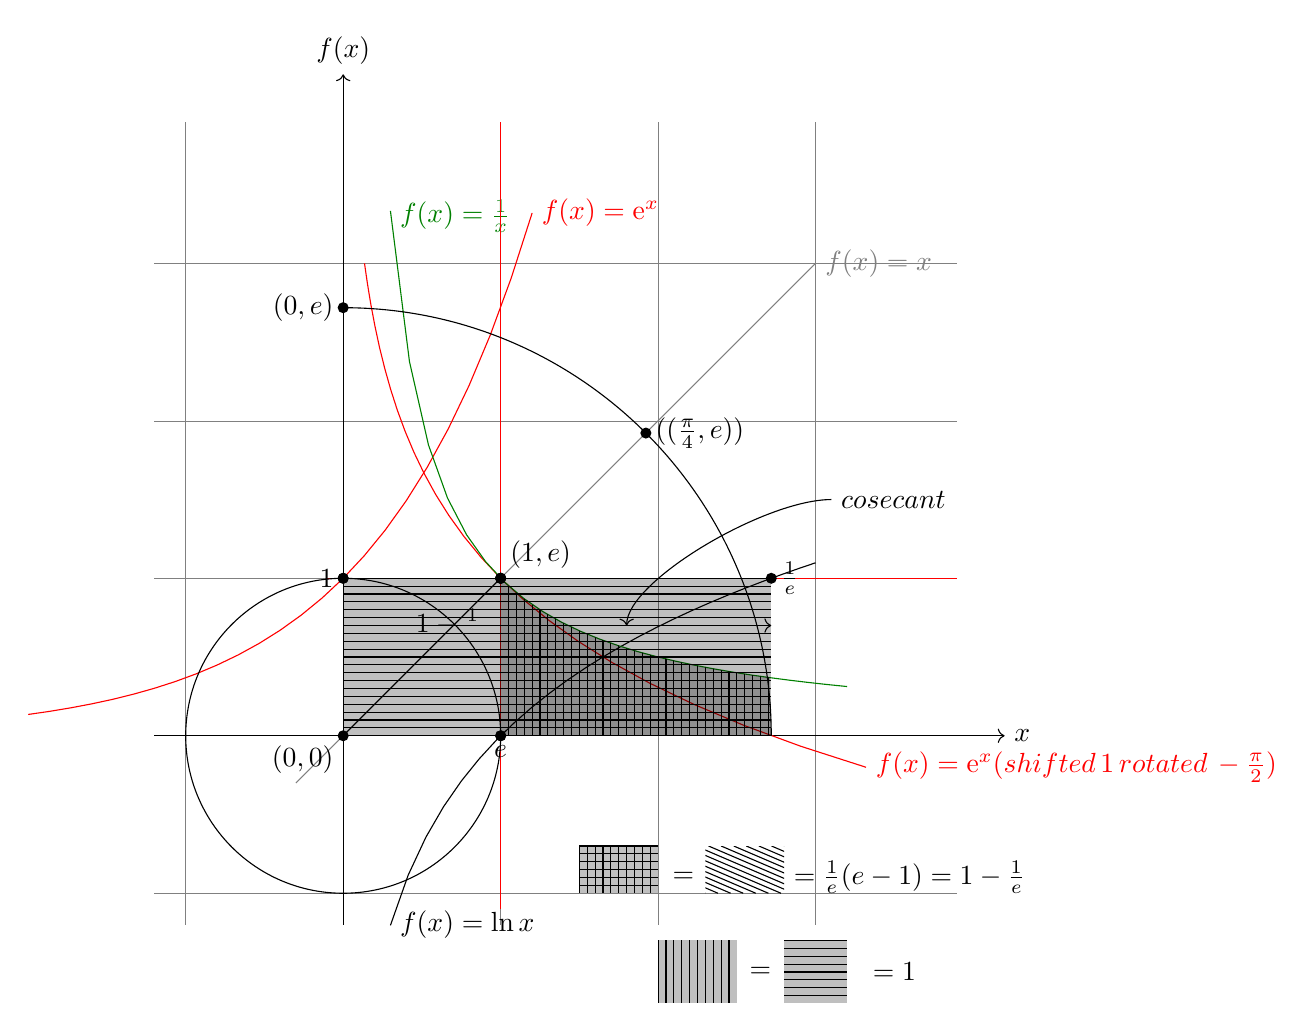
\begin{tikzpicture}[scale=2,domain=-.3:3]

 \draw[very thin,color=gray] (-1.2,-1.2) grid (3.9,3.9);
  \draw[->] (-1.2,0) -- (4.2,0) node[right] {$x$};
  \draw[->] (0,-1.2) -- (0,4.2) node[above] {$f(x)$};

  %% f(x) = x
  \draw[color=gray] plot (\x,\x) node[right] {$f(x) =x$};

  %% f(x) = ln x
  \draw[domain=.3:3,color=black] plot (\x,{ln(\x)});
  \draw[black] (.3,-1.2) node[right] {$f(x) = \ln x$};

  %% cosecant indicator
  \draw[->,black] (3.1,1.5) node[right] {$cosecant$} .. controls ++(left:12pt) and ++(up:8pt) .. (1.8,0.7);


  %% f(x) = e^x
  \draw[domain=-2:1.2,color=red]
  plot (\x,{exp(\x)}) node[right] {$f(x) = \mathrm e^x$};
  %% shifted and rotated
  \draw[domain=-2:1.2,color=red,xshift=1cm,rotate around={-90:(0,1)}]
  plot (\x,{exp(\x)}) node[right] {$f(x) = \mathrm e^x (shifted\, 1\, rotated\, -\frac{\pi}{2})$};

  %% f(x) = 1/x
  \draw[domain=.3:3.2,color=green!50!black] plot (\x,{(1/\x)});
  \draw[color=green!50!black] (.3,3.3) node[right] {$f(x) = \frac{1}{x}$};
  % \draw[] (1,.3) node[anchor=west] {$\scriptsize 1=\ln e$};

  %% (e,y) axis
  \draw[red] (\e,-1.1) -- (\e, 3.9);

  %% (x,1) axis and label
  \draw[red] (-0.1,1) -- (3.9,1);
  \fill[black] (0,1) node[left] {$1$};


  %% secant
  \draw[] (0,0) -- (\e, 1);

  %% circle
  \draw (0,0) circle (1);

  %% dot origin
  \fill[black] (0,0) node[below left] {$(0,0)$} circle (1pt);

  %% dot (0,e)
 \fill[black] (0,\inve) circle (1pt);

  %% dot (0,1)
  \fill[black] (0,1) circle (1pt);

  %% dot (1,1)
  \fill[black] (1,1) circle (1pt);

  %% dot (1, 1/e)
  \fill[black] (1, \inve) circle (1pt);

  %% label (1,e)
  \fill[black] (1,\e) node[anchor=south west] {$(1,e)$} circle (1pt);

  %% dot (e,0)
  \fill[black] (\e,0) node[below] {$e$} circle (1pt);

  %% dot (e,1)
  \fill[black] (\e,1) circle (1pt);

  %% dot (e, 1,e)
  \fill[black] ({exp(1)}, \inve) circle (1pt) node[anchor=west]
  {$\frac{1}{e}$};

  %% 1 - 1/e label
  \draw[<-] ({exp(1)}, .7) -- (\e+.4,.7) node[anchor=west] {$1-\frac{1}{\e}$};
  % \fill[black] (1,{exp(1)}) node[anchor=south west] {$(1,e)$} circle (1pt);

  %% dot (1,0)
  \fill[black] (1,0) circle (1pt);

  %% 1/x area
  \begin{scope}[domain=1:2.71]
    \clip (1,0)--(1,1) -- plot (\x,{(1/\x)}) -- ({exp(1)},0) -- cycle;
    \fill[opacity=.25] (1,0) -- ({exp(1)},0) -- ({exp(1)},1) -- (1,1);
    \foreach \step in {0,.05,...,4} {
      \pgfmathsetmacro\inc{\step}
      \draw (1+\inc,0) -- (1+\inc,1);
    }
  \end{scope}

  %% area lines
  \fill[opacity=.25] (2,-1.3) rectangle (2.5,-1.7);
  \foreach \step in {0,.05,...,.5} {
    \draw (2+\step,-1.3cm) -- (2+\step,-1.7);
  }

  \draw (2.65,-1.5) node {$=$};

  \fill[opacity=.25] (2.8,-1.3) rectangle (3.2,-1.7);
  \foreach \step in {0,.05,...,.4} {
    \draw (2.8,-1.3-\step) -- (3.2,-1.3-\step);
  }
  %% end 1/x area

  \def\eul{{exp(1)}};
  \def\inveul{\inve};
  %% upper square area lines
  \begin{scope}
    \clip (0,0) rectangle (1,1);
    %% \fill[opacity=.25] (0,0) -- ({exp(1)},0) -- ({exp(1)}, \inve) -- (0,\inve) -- cycle;
    \foreach \step in {0,.07,...,2.5} {
      \pgfmathsetmacro\inc{\step}
      \draw (\step,\inveul) -- (\step-.7,1);
      % \draw (-.5+\inc,0) -- (\inc+3,{exp(1)});
    }
  \end{scope}

  %% area key
  \fill[opacity=.25] (1.5,-.7) rectangle (2,-1);
  \foreach \step in {0,.05,...,.5} {
    %% v lines
    \draw (1.5+\step,-.7) -- (1.5+\step,-1);
  }

  \draw (2.03,-.9) node[anchor=west] {$=$};

  \foreach \step in {0,.05,...,.3} {
    %% h lines
    \draw (1.5,-.7-\step) -- (2,-.7-\step);
  }

  %% slant lines key
  %% \fill[opacity=.25] (2.3,-.7) rectangle (2.8,-1);
  \begin{scope}
    \clip (2.3,-.7) rectangle (2.8,-1);
    %% \fill[opacity=.25] (0,0) -- ({exp(1)},0) -- ({exp(1)}, \inve) -- (0,\inve) -- cycle;
    \foreach \step in {1.6,1.68,...,2.8} {
      \pgfmathsetmacro\inc{\step}
      \draw (\step,-.7) -- (\step+.7,-1);
      % \draw (-.5+\inc,0) -- (\inc+3,{exp(1)});
    }
  \end{scope}

  \draw (2.8,-.9) node[anchor=west] {$= \frac{1}{e}(e-1) = 1-\frac{1}{e}$};

  %%
  \draw (3.5,-1.5) node {$= 1$};

  %% e rectangle
  %% PATTERNS seem to be broken
  %% \draw[pattern=dots] (0,0) -- ({exp(1)},0) -- ({exp(1)}, \inve) -- (0,\inve) -- cycle;
  \begin{scope}
    \clip (0,0) -- ({exp(1)},0) -- ({exp(1)}, \inve) -- (0,\inve) -- cycle;
    \fill[opacity=.25] (0,0) -- ({exp(1)},0) -- ({exp(1)}, \inve) -- (0,\inve) -- cycle;
    \foreach \step in {0,.05,...,4} {
      \pgfmathsetmacro\inc{\step}
      \draw (0,\inc) -- ({exp(1)},\inc);
      % \draw (-.5+\inc,0) -- (\inc+3,{exp(1)});
    }
  \end{scope}

  %% e radius (= focus of hyperbola?)

%  \newlength{\gnat}
%  \setlength{\gnat}{{\eul}*1cm}
  \pgfmathsetmacro\e{exp(1) * 1cm}
%  \pgfmathparse{exp(1)cm} \pgfmathresult \let\e\pgfmathresult
  \draw (\eul,0) arc (0:90:\eul);
  \fill (canvas polar cs:angle=45,radius=\e) circle (1pt) node[anchor=west] {($(\frac{\pi}{4},e)$)};
  \fill (0,\eul) circle (1pt) node[anchor=east] {($0,e$)};

  %% arc e
  draw (1,0) arc (e:1);

\end{tikzpicture}
\end{figure}

%%% Local Variables: 
%%% mode: latex
%%% TeX-master: t
%%% End: 

%%%%%%%%%%%%%%%%%%%%%%%%%%%%%%%%%%%%%%%%%%%%%%%%%%%%%%%%%%%%%%%%
%%  e sector
\begin{figure}[ht]
\begin{tikzpicture}[scale=2,domain=-.3:3]

 \draw[very thin,color=gray] (-1.2,-1.2) grid (3.9,3.9);
  \draw[->] (-1.2,0) -- (4.2,0) node[right] {$x$};
  \draw[->] (0,-1.2) -- (0,4.2) node[above] {$f(x)$};

  % shade e sector
  \begin{scope}[domain=1:\e]
    \clip (0,0)--(1,1) -- plot (\x,{(1/\x)}) -- (\e,\inve) -- cycle;
    \fill[opacity=.25] (0,0) -- (\e,0) -- (\e,1) -- (0,1);
%    \foreach \step in {0,.05,...,4} {
%      \pgfmathsetmacro\inc{\step}
%      \draw (1+\inc,0) -- (1+\inc,1);
%    }
  \end{scope}

 %% axis:  f(x) = x
%  \draw[color=gray] plot (\x,\x) node[right] {$f(x) =x$};
  \draw[color=gray] (0,0) -- (3.2,3.2) node[right] {$f(x) =x$};
  \draw[black] (0,0) -- (1,1);

%% f(x) = 1/x
  \draw[domain=.3:3.2,color=green!50!black] plot (\x,{(1/\x)});
  \draw[color=green!50!black] (.3,3.3) node[right] {$f(x) = \frac{1}{x}$};
  % \draw[] (1,.3) node[anchor=west] {$\scriptsize 1=\ln e$};

  %% (e,y) axis
  \draw[red, dashed] (\e,-1.1) -- (\e, 3.9);
  %% (x,e) axis
  \draw[red, dashed] (0,\e) -- (3.9,\e);

  %% (x,1) axis and label
  \draw[red, dashed] (-0.1,1) -- (3.9,1);
  \fill[black] (0,1) node[left] {$1$};

  %% secant
  \draw[dashed] (0,0) -- (\e, 1);

  %% e diameter
  \draw[black] (0,0) -- (\e, \inve);

  %% circle
  \draw (0,0) circle (1);

  \draw[gray] (1/\sqrttwo,0) node[below] {$\frac{1}{\sqrt{2}}$}
  -- (1/\sqrttwo,1/\sqrttwo);
  \draw[gray] (0,1/\sqrttwo) -- (1/\sqrttwo,1/\sqrttwo);

  \draw[gray] (\sqrttwo,0) node[below left] {$\scriptsize\sqrt{2}$}
  -- (\sqrttwo,\sqrttwo);
  \draw[gray] (0,\sqrttwo) -- (\sqrttwo,\sqrttwo);

  %%%%
  \draw[gray] (0,e/\sqrttwo) -- (e/\sqrttwo,e/\sqrttwo);
 \draw[gray] (e/\sqrttwo,0) node[below] {$\frac{e}{\small\sqrt{2}}$}
  -- (e/\sqrttwo,e/\sqrttwo);

  %%%%
  \draw[gray] (0,3/2) node[left] {$\frac{3}{2}$} -- (3/2,3/2);
  \draw[gray] ({2-\sqrttwo+1},0) node[below=10pt] {$2-\frac{1}{e}$} -- ({2-\sqrttwo+1},{2-\sqrttwo+1});

  %% dot origin
  \fill[black] (0,0) node[below left] {$O$} circle (.7pt);

  %% dot (0,1/e)
 \fill[black] (0,\inve) circle (.7pt);

  %% dot (0,1)
  \fill[black] (0,1) node[above right] { $A$}  circle (.7pt);

  %% dot (1,1)
  \fill[black] (1,1) node[above right] { $B$}  circle (.7pt);

 %% label (1,e)
  \fill[black] (1,\e) node[anchor=south west] {$(1,e)$} circle (.7pt);

 %% segment
  \draw[black] (1,1) -- (e,1/e);

 %% dot (e,1)
  \fill[black] (\e,1) node[above right]  {$C$} circle (.7pt); 

  %% dot (e,0)
  \fill[black] (\e,0) node[below right]{$E$} node[below] {$e$} circle (.7pt);

  %% dot (0, 1/e)
  \fill[black] (0, \inve) circle (.7pt) node[left]  {$\frac{1}{e}$}
  node[right] {$F$};

  %% dot (e, e)
  \fill[red] (\e, e) circle (.7pt) node[below right]  {$(e,e)$};


  %% 1 - 1/e label
  \draw (\e,0) -- (\e,1);
%  \draw[<-] (\e, .7) -- (\e+.4,.7) node[anchor=west] {$1-\frac{1}{e}$};
  % \fill[black] (1,\e) node[anchor=south west] {$(1,e)$} circle (.7pt);

  %% dot (1,0)
  \fill[black] (1,0) circle (.7pt);

 \draw (\e,0) arc (0:90:\e);
 \fill (canvas polar cs:angle=45,radius=2.71cm) circle (.7pt)
 node[right] {$P$};
 \fill (canvas polar cs:angle=30,radius=2.71cm)
 node[right]{$\frac{\pi\,e}{4} = PE$};

%  \fill (0,\e) circle (.7pt) node[anchor=east] {($0,e$)};

  %% dot (0, 1/e)
  \fill[black] (1, \inve) circle (.7pt);
 %% dot (e, 1/e)
  \fill[black] (\e, \inve) node[right] {$D$} circle (.7pt);
  \draw[gray] (0,\inve) -- (\e,\inve);

\end{tikzpicture}
\caption{e sector}
\end{figure}

%%% Local Variables: 
%%% mode: latex
%%% TeX-master: t
%%% End: 


\noindent
\end{document}
